\documentclass[10pt]{beamer} % beamer format
\usepackage[utf8]{inputenc}  % spanish package 

\usetheme[progressbar=frametitle]{metropolis} % beamer theme
\usepackage{appendixnumberbeamer}

\usepackage{booktabs}
\usepackage[scale=2]{ccicons}

\usepackage{epstopdf}
\usepackage{graphicx} % graphics package
\usepackage{subfig}	  % package for multiple figure
\usepackage[justification=centering]{caption}

\usepackage{xcolor}
\usepackage{enumerate}

\definecolor{darkblue}{HTML}{4f81bd}
\definecolor{darkyellow}{HTML}{bf9000}

\newcommand{\themename}{\textbf{\textsc{metropolis}}\xspace}




\begin{document}

	\title{PD-SMC controller parameter optimization oriented to improved performance in surgical tasks}
	\date{}
	\author{Jhon Charaja, Emanuel Muñoz-Panduro, Oscar E. Ramos, and Ruth Canahuire
	}
	\institute{Department of Mechatronics Engineering, Universidad de Ingeniería y Tecnología - UTEC}
	
	\frame{\titlepage}
	
	\section{Proceso de optimización}
	
	\begin{frame}[fragile]{Función costo}
		La función costo se formula de la siguiente manera:
		\begin{align*}
			J &= \frac{\gamma}{2}\mathrm{P_1}^2 + \frac{\beta}{2}\mathrm{P_2}^2, \\
			1 &= \gamma + \beta,
		\end{align*}
		donde
		\begin{align*}
			\bullet \textrm{ }\mathrm{P_1} &: f(\textrm{ganancia de control, error en posición y velocidad}). \\
			\bullet \textrm{ }\mathrm{P_2} &: f(\textrm{error en jerk}). \\
		\end{align*}
	\end{frame}

	\begin{frame}[fragile]{Descenso de gradiente}
		La variable de control ($k$) se actualiza de la siguiente manera:
		\begin{align*}
			k := k - \alpha \frac{\partial J}{\partial k},
		\end{align*}
		la gradiente se calcula como sigue:
		\begin{align*}
			\frac{\partial J}{\partial k} &= \frac{\partial J}{\partial y} \frac{\partial y}{\partial u} \frac{\partial u}{\partial k}, 
		\end{align*}
		donde 
		\begin{align*}
			\bullet \textrm{ } \alpha&: \textrm{tasa de aprendizaje.} \\			
			\bullet \textrm{ } J&: \textrm{función costo.} \\
			\bullet \textrm{ } y&: \textrm{salida del sistema.} \\
			\bullet \textrm{ } u&: \textrm{ley de control.} \\
			\bullet \textrm{ } k&: \textrm{ganancia de control.}
		\end{align*}
	\end{frame}
			
	

	
	\section{Métodos de control}

	\begin{frame}[fragile]{control de modo deslizante}	
	La ley de control en el espacio articular se define de la siguiente manera:
	\begin{align*}
		u &= M \left[\ddot{q}_d + s + \mathrm{tanh}(s) \right] + b,
	\end{align*}
	con
	\begin{align*}
		s &= 2 \lambda \dot{e} + \lambda^2 e, \\
		e &= q_d - q,
	\end{align*} 
	donde
		\begin{align*}
			\bullet \textrm{ } M&: \textrm{Matriz de inercia.} 			\\
			\bullet \textrm{ } \lambda&: \textrm{ganancia de control.} 	\\
			\bullet \textrm{ } s&: \textrm{variable de deslizamiento.} 	\\
			\bullet \textrm{ } b&: \textrm{Vector de efectos no lineales.}							
		\end{align*}
	\end{frame}	
	
	\begin{frame}[fragile]{Control de modo deslizante}	
		Las parámetros de la función costo se definen de la siguiente manera:
		\begin{align*}
			\mathrm{P_1}&= s, \\
			\mathrm{P_2}&= \dot{s}(2 - \mathrm{tanh}^2(s)),
		\end{align*}
		La gradiente y las derivadas de la función costo:
		\begin{align*}
			 \frac{\partial J}{\partial \lambda} &= \left(\gamma \mathrm{P_1} \frac{\partial \mathrm{P_1}}{\partial q} + \beta \mathrm{P_2} \frac{\partial \mathrm{P_2}}{\partial q} \right)
			 \frac{\partial u}{\partial \lambda}, \\
			 \frac{\partial \mathrm{P_1}}{\partial q} &= -\lambda^2, \\
			 \frac{\partial \mathrm{P_2}}{\partial q} &= -2\lambda\dot{\lambda}(2-\mathrm{tanh}^2(s)) + 2\dot{s}\lambda^2 \mathrm{tanh}(s) (1-\mathrm{tanh}^2(s)), \\
			 \frac{\partial u}{\partial \lambda} &= 2M \left[(\dot{e}+\lambda e)(2- \mathrm{tanh}^2(s) ) \right]
		\end{align*}
		
	\end{frame}

	\begin{frame}[fragile]{Control proporcional-derivativo}
	La ley de control en el espacio articular se define de la siguiente manera:
	\begin{align*}
		u &= M \left[\ddot{q}_d + k_p e + k_d \dot{e} \right] + b,
	\end{align*}
	con
	\begin{align*}
		e &= q_d - q,
	\end{align*} 
	donde
	\begin{align*}
		\bullet \textrm{ } M&: \textrm{Matriz de inercia.} 			\\
		\bullet \textrm{ } k_p&: \textrm{ganancia proporcional.} 	\\
		\bullet \textrm{ } k_d&: \textrm{ganancia derivativa.} 	\\
		\bullet \textrm{ } b&: \textrm{Vector de efectos no lineales.}							
	\end{align*}		
	\end{frame}

	\begin{frame}[fragile]{Control proporcional-derivativo}
	Las parámetros de la función costo se definen de la siguiente manera:
	\begin{align*}
		\mathrm{P_1}&=  k_p e + k_d \dot{e}, \\
		\mathrm{P_2}&= \dot{k}_p e + k_p \dot{e} +\dot{k}_d\dot{e} + k_d\ddot{e},
	\end{align*}
	La gradiente respecto a cada ganancia de control:
	\begin{align*}
		%\frac{\partial J}{\partial k} &= \left(\gamma \mathrm{P_1} \frac{\partial \mathrm{P_1}}{\partial q} + \beta \mathrm{P_2} \frac{\partial \mathrm{P_2}}{\partial q} \right) \frac{\partial u}{\partial k}, \\
		\frac{\partial J}{\partial k_p} &= (-\gamma\mathrm{P_1}k_p - \beta\mathrm{P_2}\dot{k}_p)(Me), \\
		\frac{\partial J}{\partial k_d} &= (-\gamma\mathrm{P_1}k_p - \beta\mathrm{P_2}\dot{k}_p)(M\dot{e}).
	\end{align*}		
	\end{frame}

	\section{Resultados}
	\begin{frame}[fragile]{Parámetros de la primera simulación ($60$ segundos)}
		\begin{minipage}{\textwidth}
			\large \color{darkblue}{\textbf{Datos del controlador}} 
			\begin{itemize}
				\item Se realizan simulaciones para: $\alpha=0.1$, $0.5$, $0.8$.
				
				\item Se mantiene constante: $\gamma=0.999$ y $\beta=0.001$.
				
				\item La ganancia de control se inicia con: $\lambda=0.5$.
			\end{itemize}
		\color{white}{para crear espacio, borrar luego}	 
		\end{minipage}
	
		\begin{minipage}{\textwidth}		
			\large \color{darkblue}{\textbf{Datos de la trayectoria}}
			\begin{itemize}
				\item Trayectoria circular de radio $0.5$ m en el plano XY.
				
				\item Trayectoria sinusoidal de amplitud $0.2$ m en el eje Z.
				
				\item El periodo de las trayectorias es $10$ segundos.
			\end{itemize}
		\end{minipage}		
	\end{frame}
	
	
	\begin{frame}[fragile]{Control de modo deslizante}
		\begin{figure}
			\centering
			\hspace*{-0.7cm}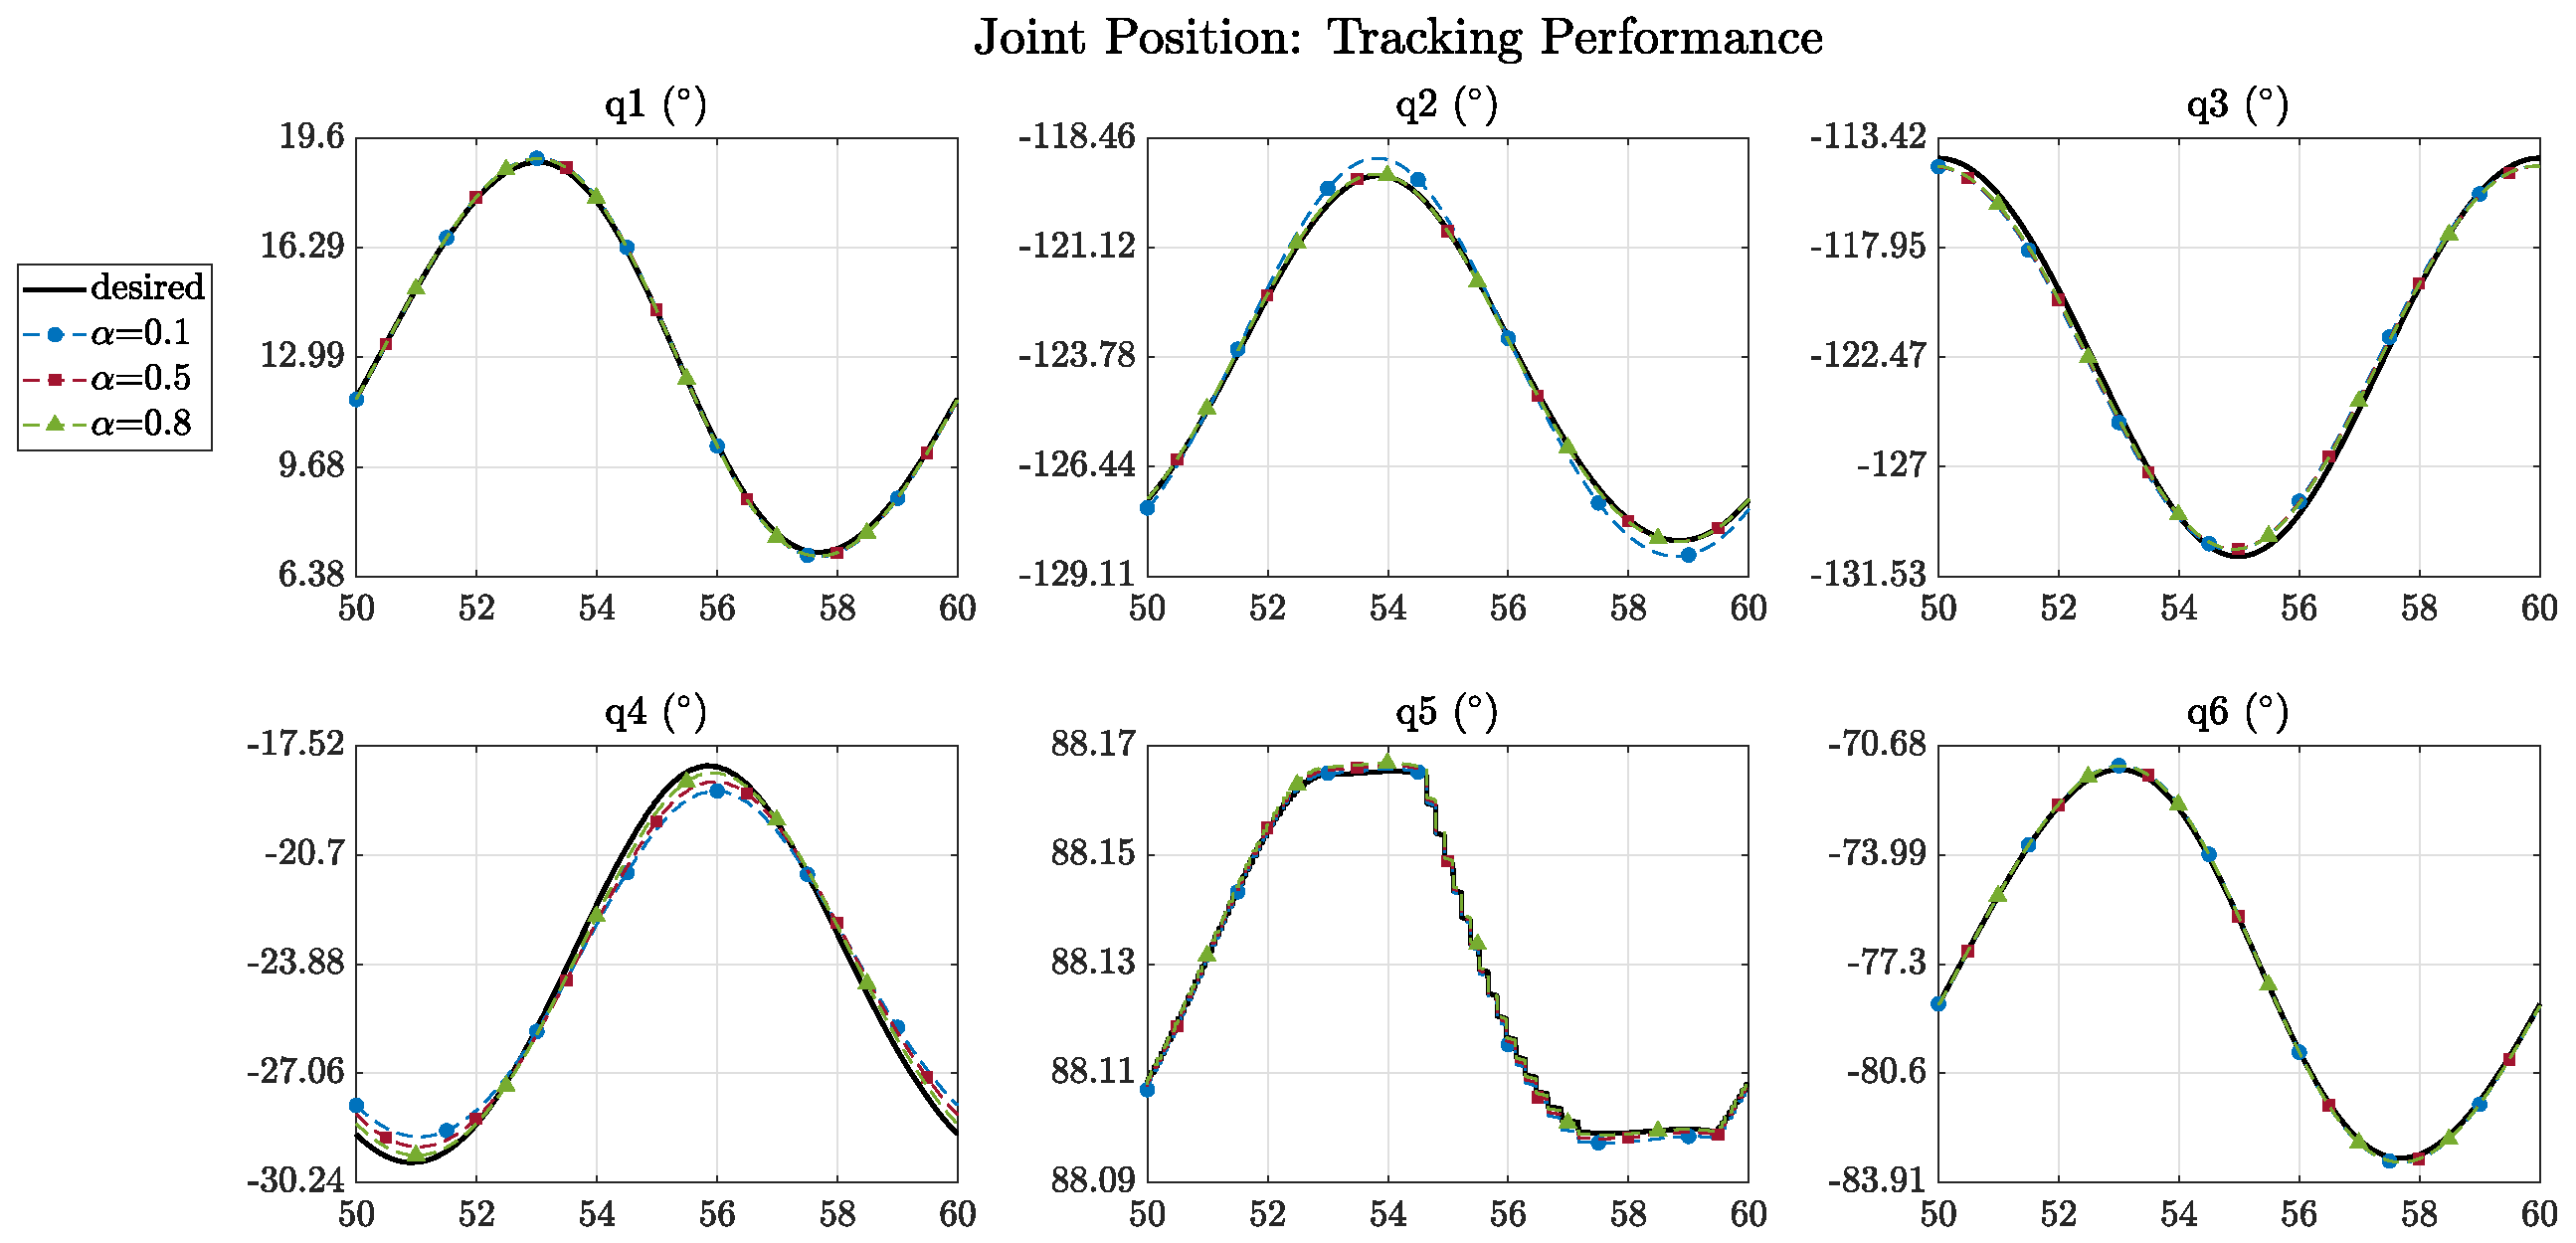
\includegraphics[width=1.1\textwidth]{img/SMCi/circular_traj/60_seg/articular_SMCi_position_compare.eps}
		\end{figure}
	\end{frame}
	
	\begin{frame}[fragile]{Control de modo deslizante}
		\begin{figure}
			\centering
			\hspace*{-0.7cm}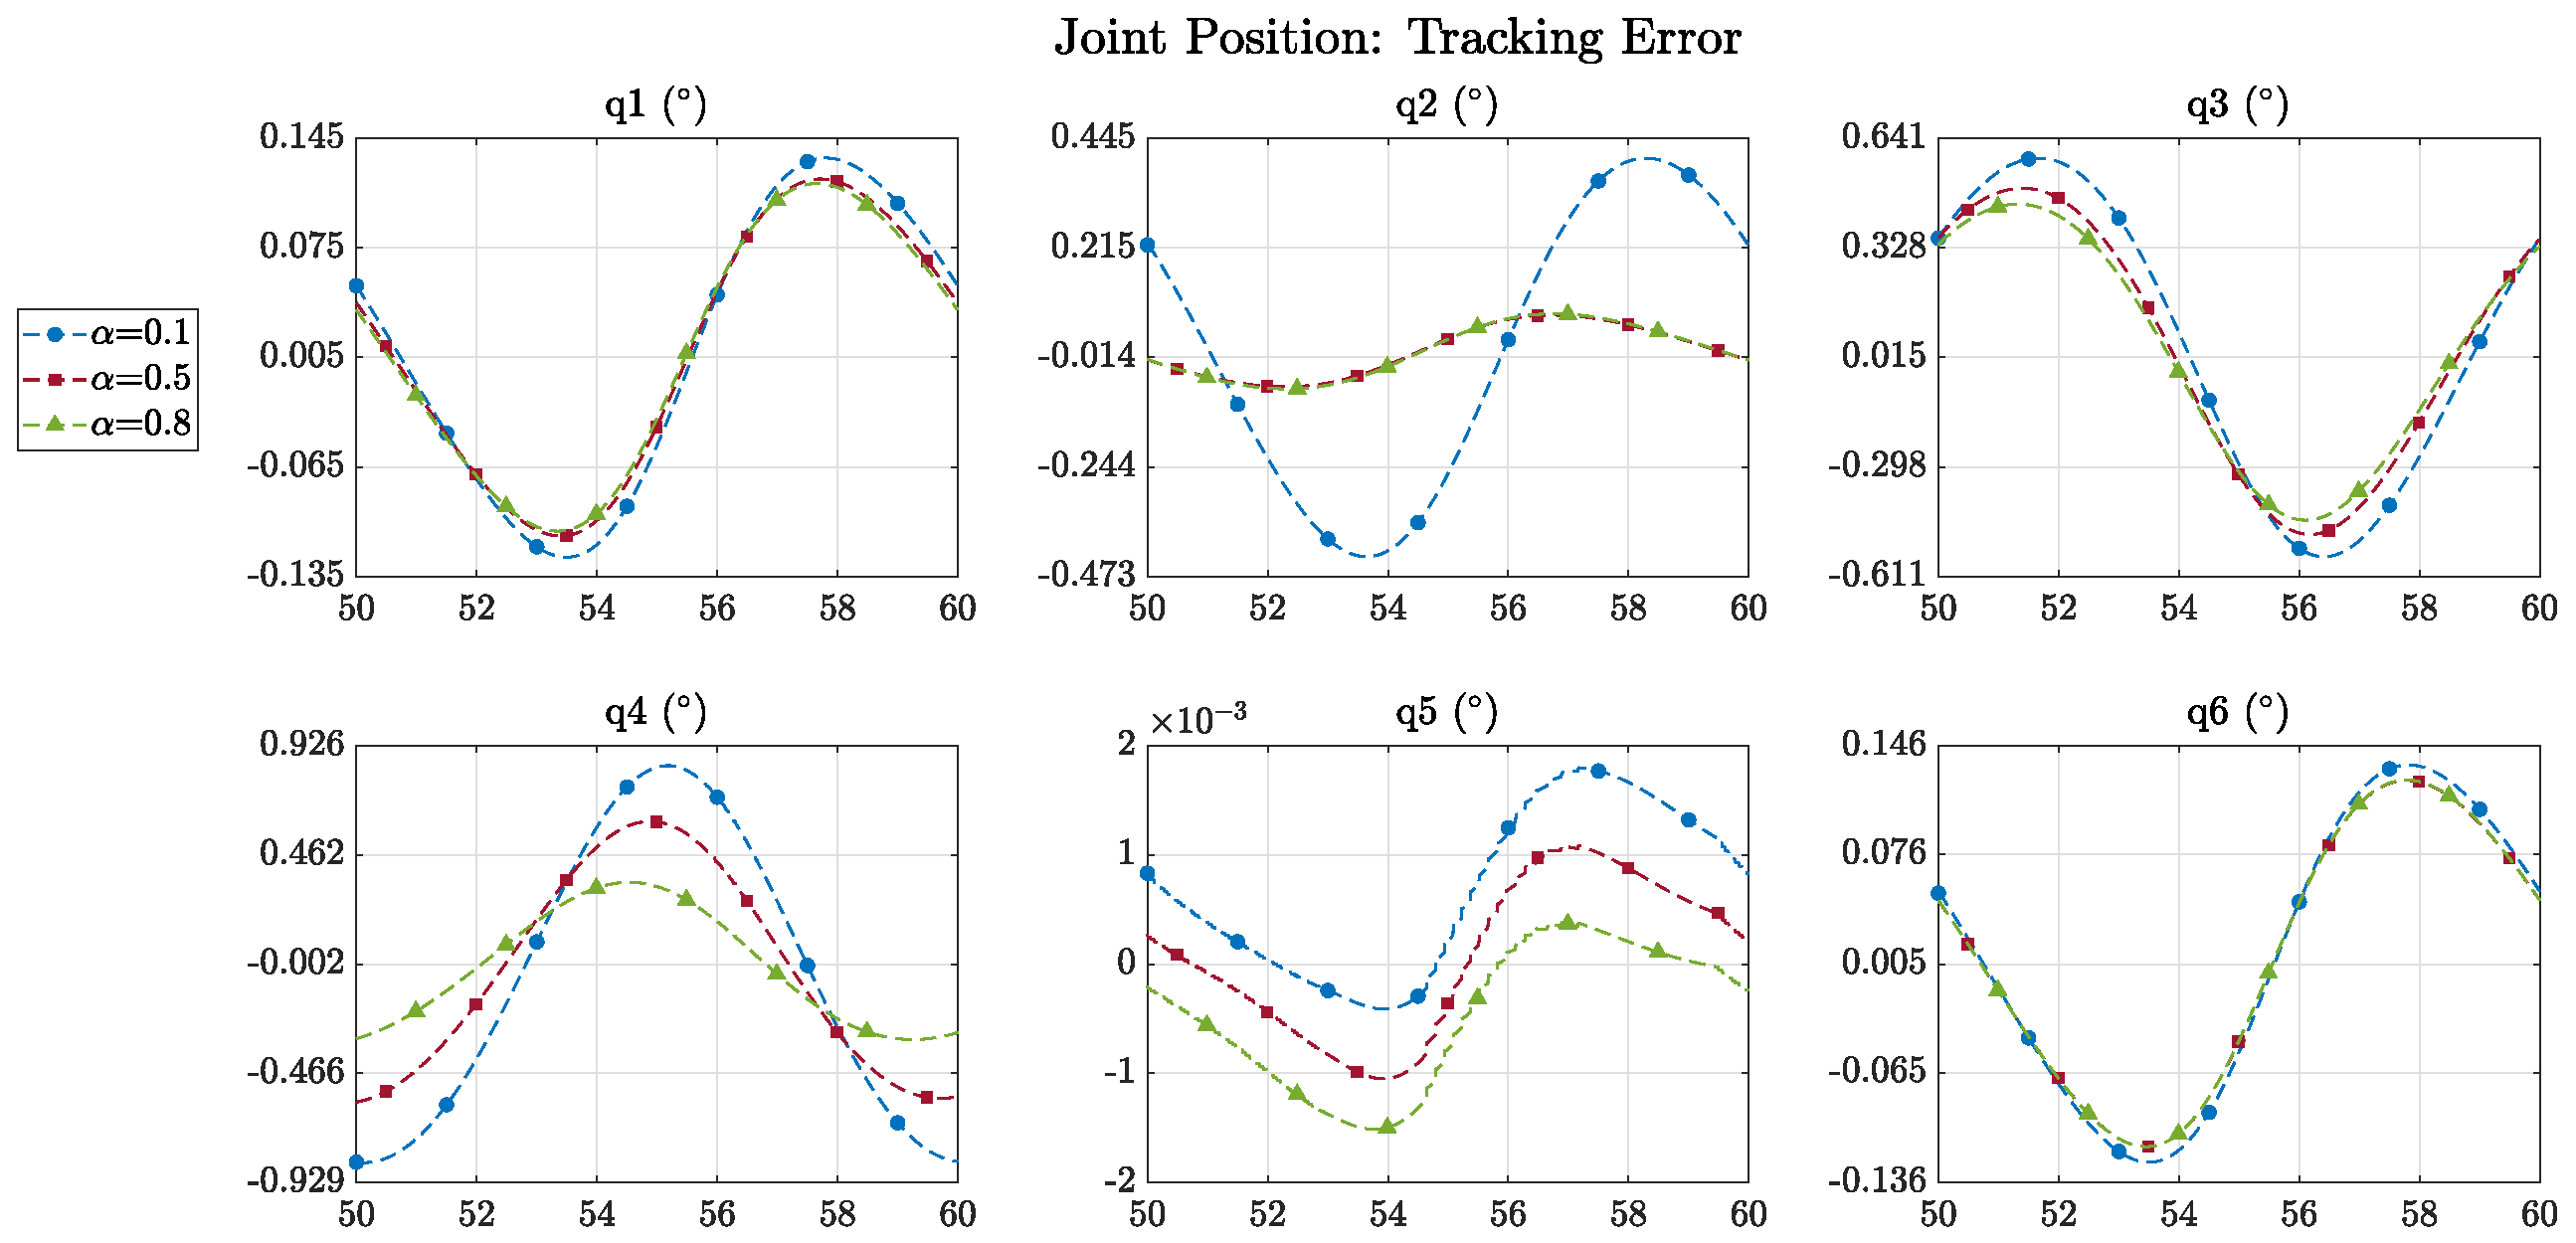
\includegraphics[width=1.1\textwidth]{img/SMCi/circular_traj/60_seg/articular_SMCi_position_error_compare.eps}
		\end{figure}
	\end{frame}	
	
	\begin{frame}[fragile]{Control de modo deslizante}
		\begin{figure}
			\centering
			\hspace*{-0.7cm}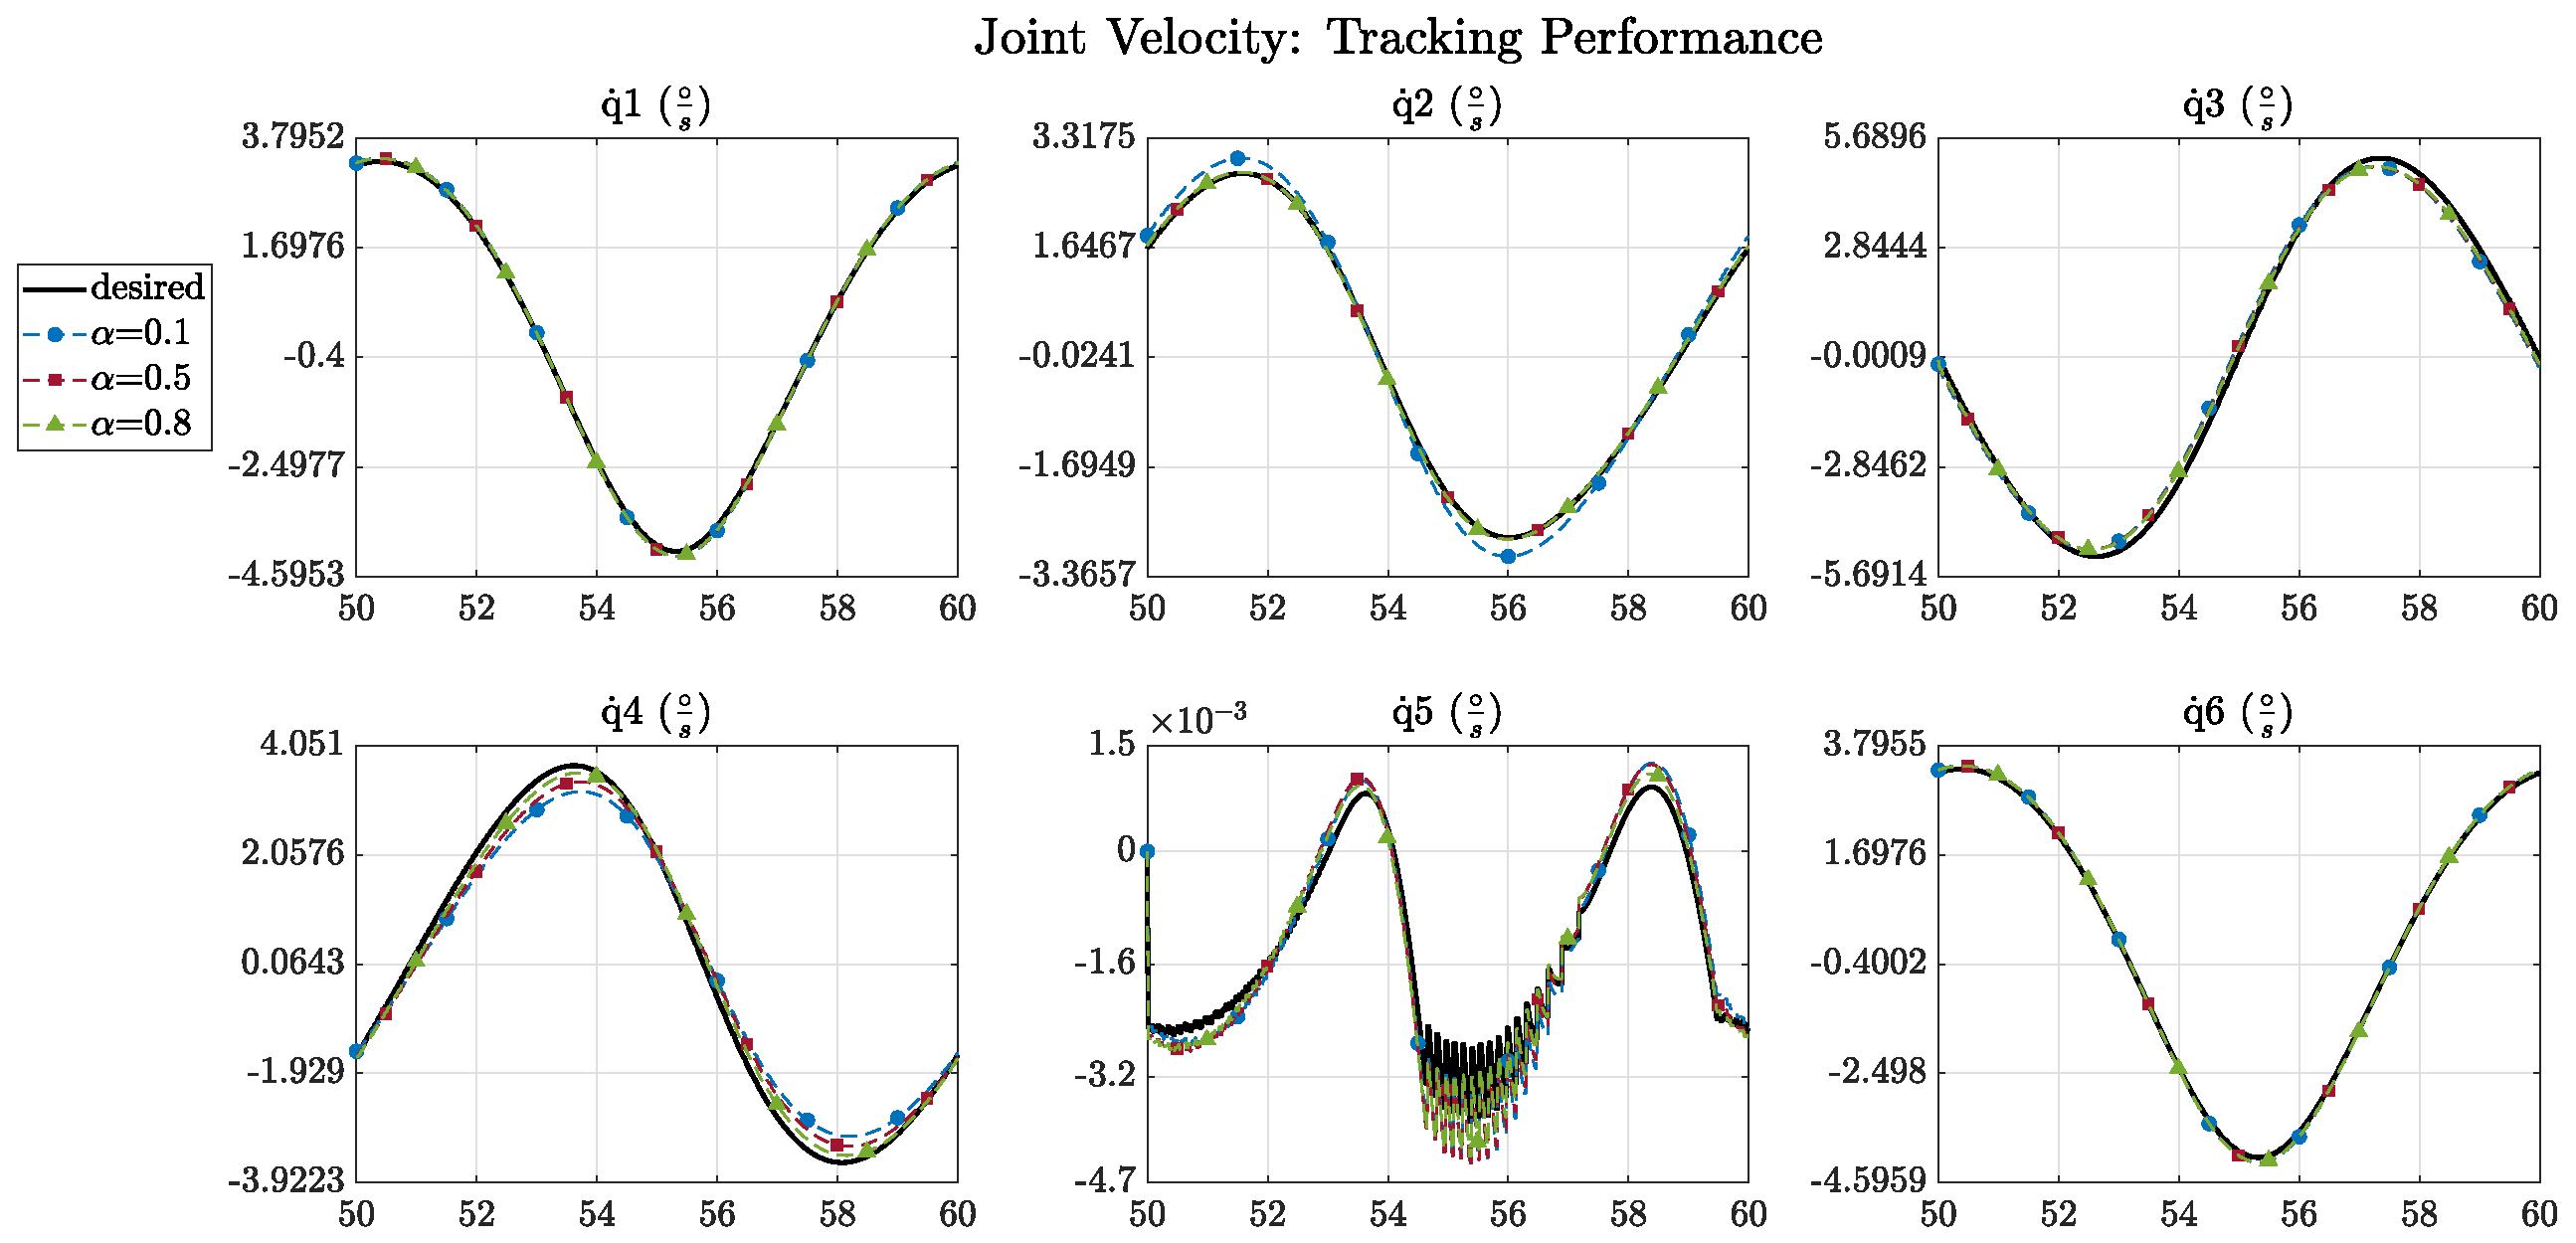
\includegraphics[width=1.1\textwidth]{img/SMCi/circular_traj/60_seg/articular_SMCi_velocity_compare.eps}
		\end{figure}
	\end{frame}

	\begin{frame}[fragile]{Control de modo deslizante}
		\begin{figure}
			\centering
			\hspace*{-0.7cm}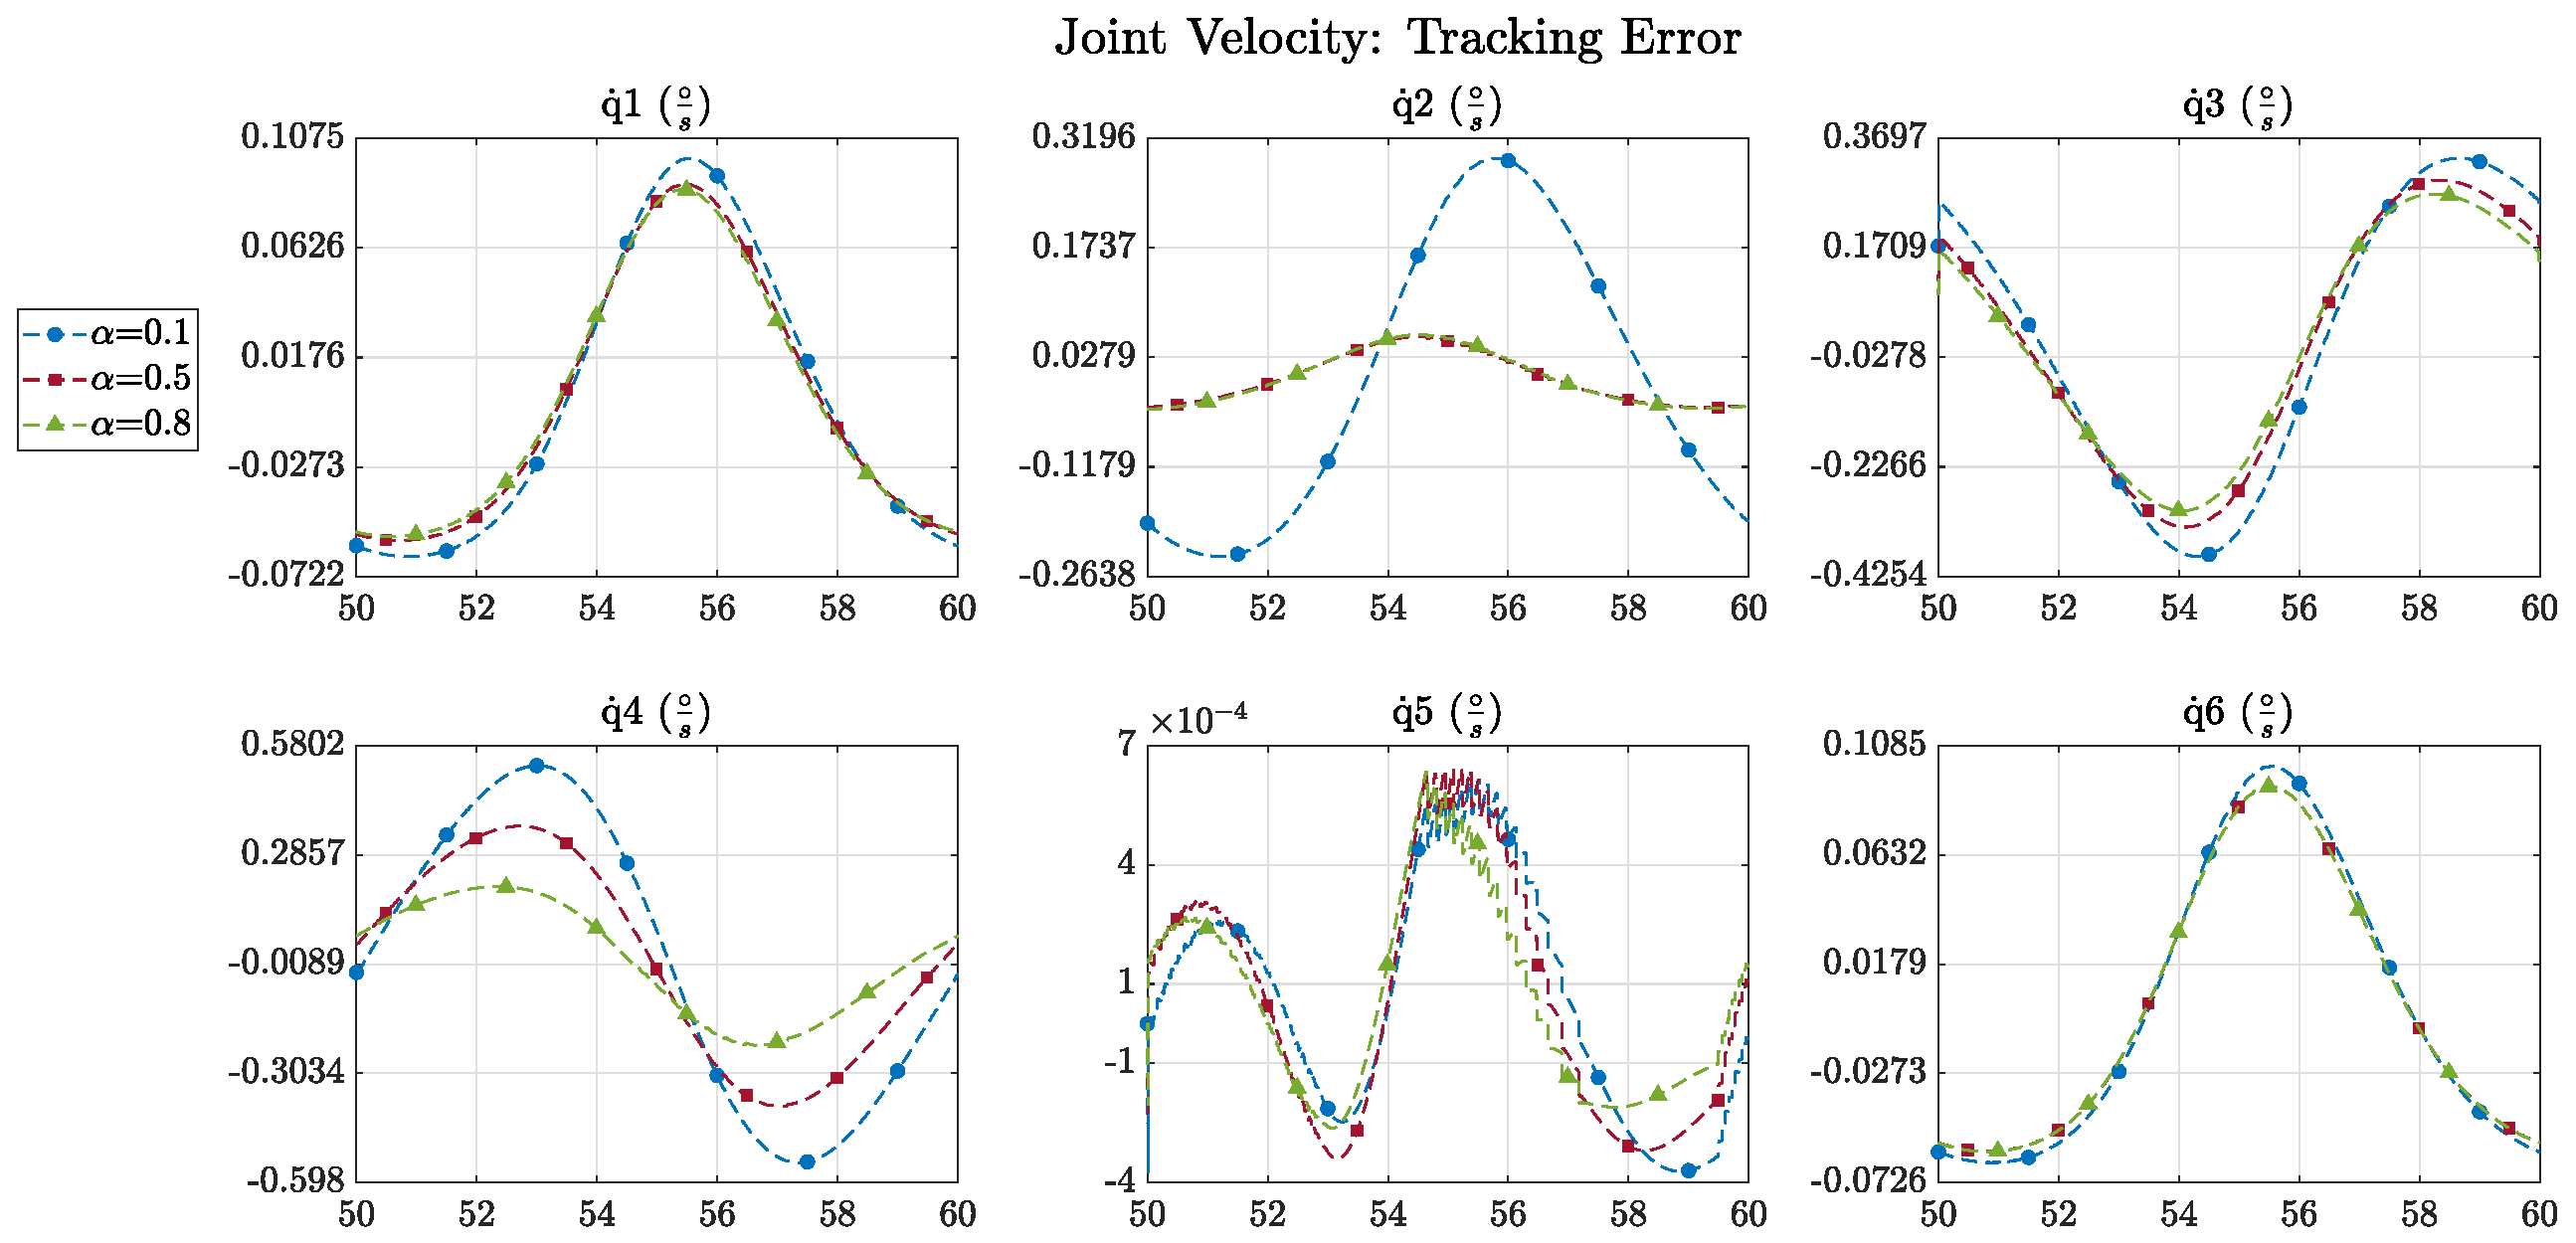
\includegraphics[width=1.1\textwidth]{img/SMCi/circular_traj/60_seg/articular_SMCi_velocity_error_compare.eps}
		\end{figure}
	\end{frame}

	\begin{frame}[fragile]{Control de modo deslizante}
		\begin{figure}
			\centering
			\hspace*{-0.5cm}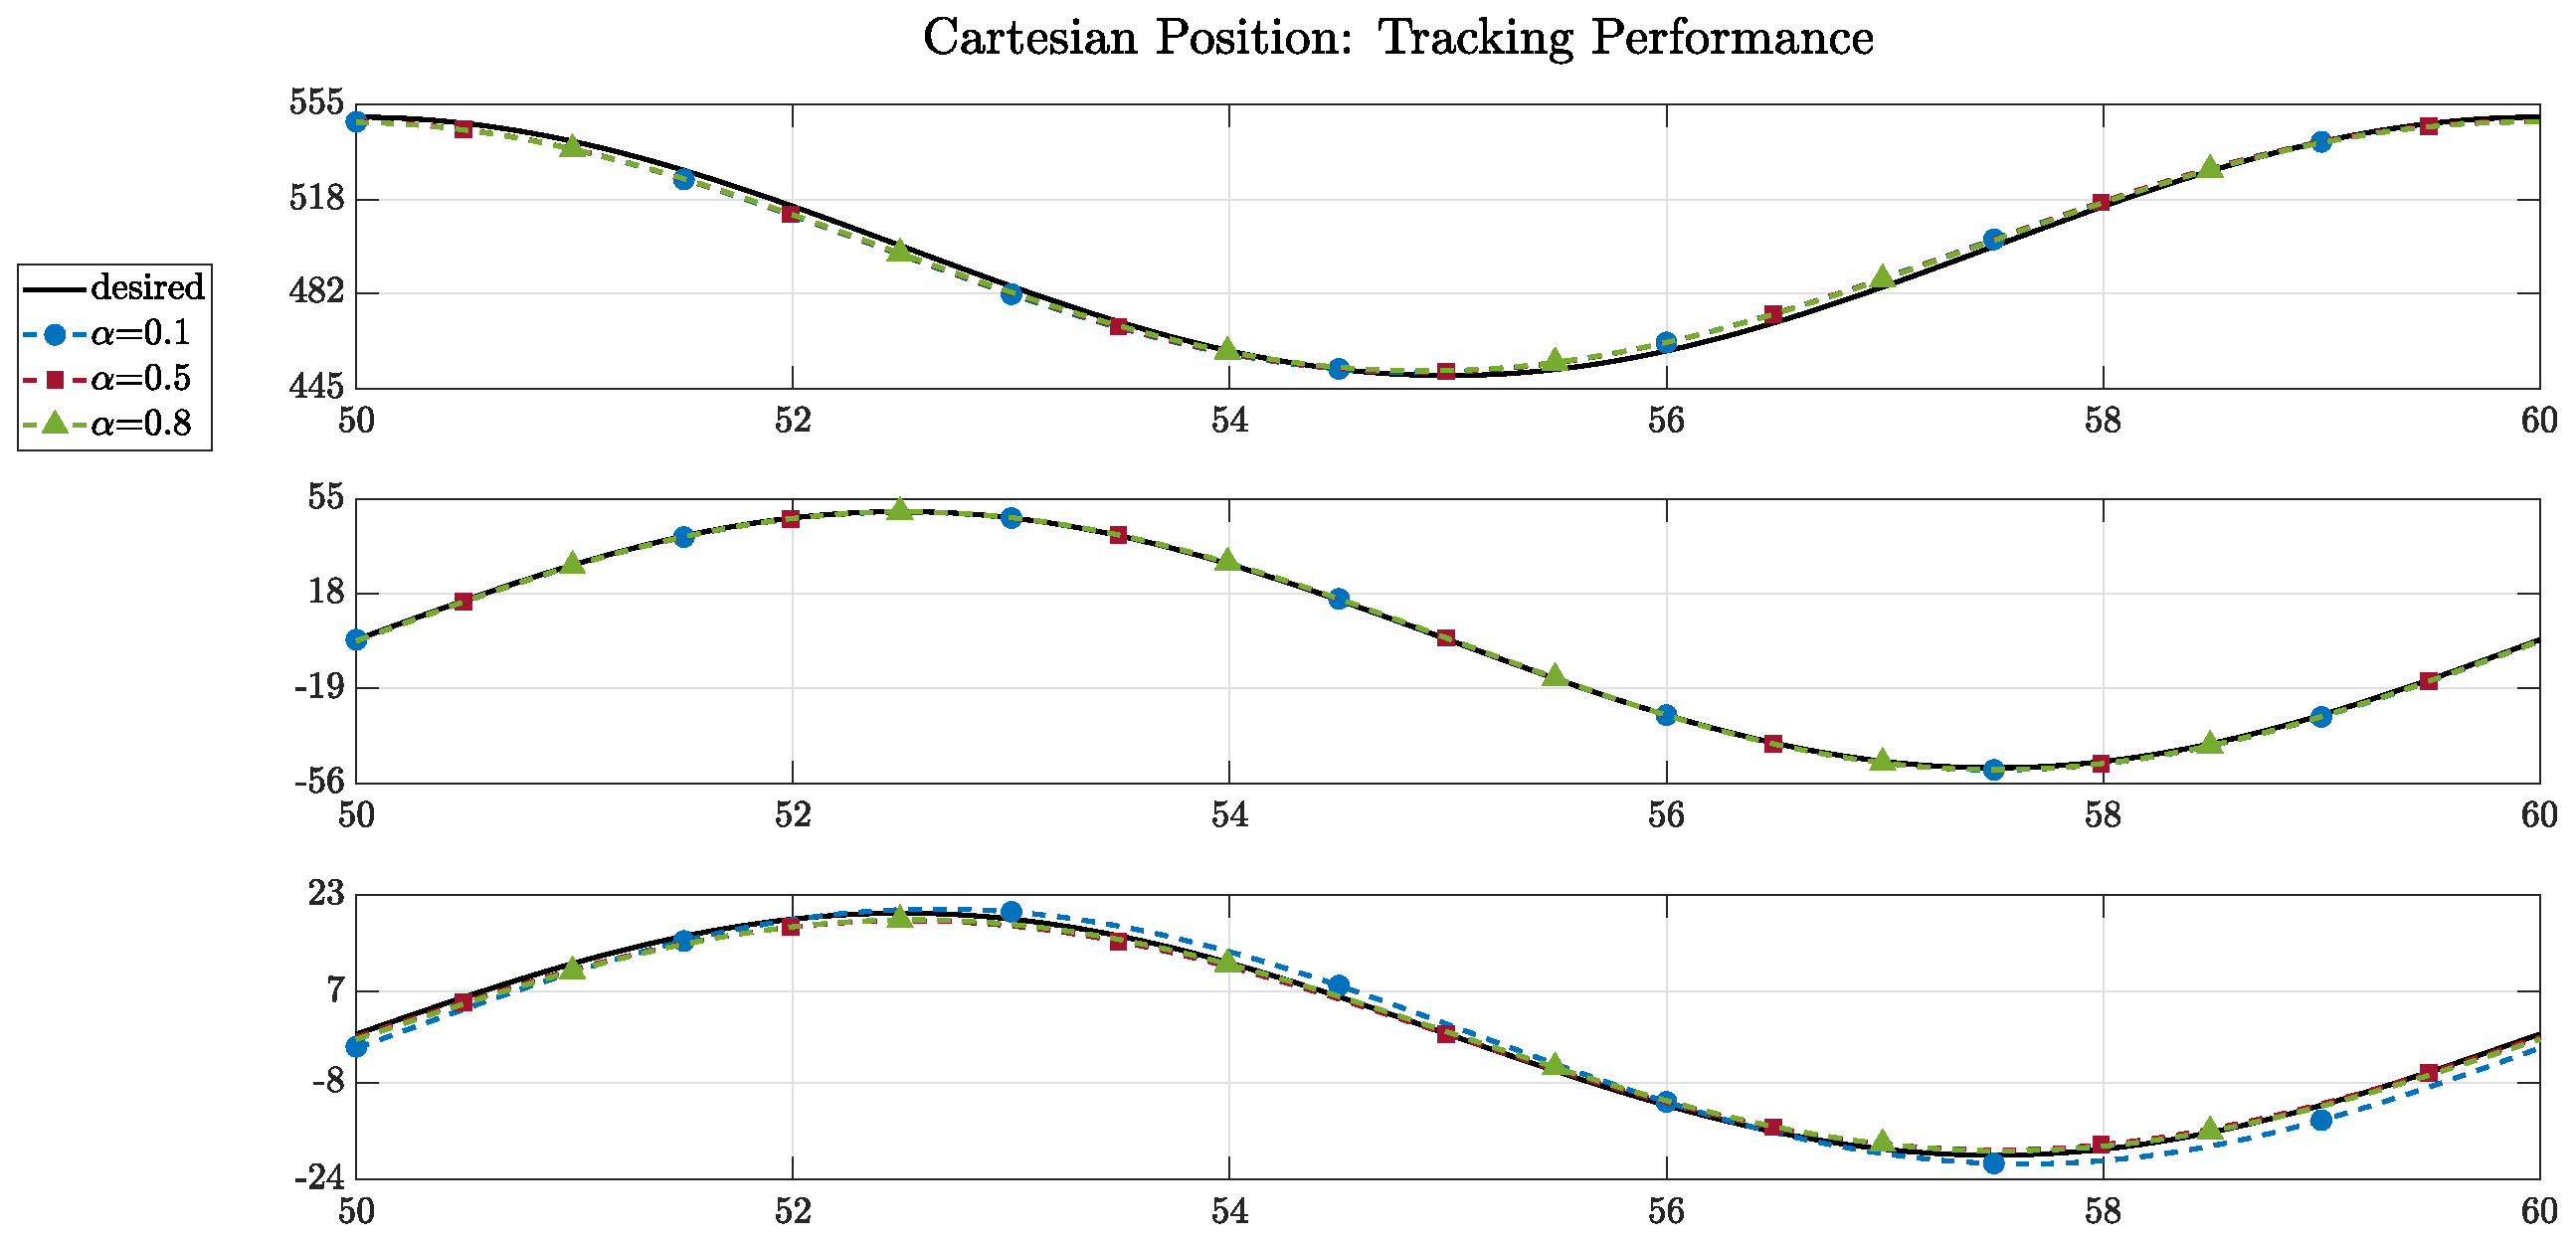
\includegraphics[width=1.1\textwidth]{img/SMCi/circular_traj/60_seg/articular_SMCi_pos_xyz_compare.eps}
		\end{figure}
	\end{frame}

	\begin{frame}[fragile]{Control de modo deslizante}
		\begin{figure}
			\centering
			\hspace*{-0.5cm}\includegraphics[width=1.1\textwidth]{img/SMCi/circular_traj/60_seg/articular_SMCi_pos_xyz_error_compare.eps}
		\end{figure}
	\end{frame}

	\begin{frame}[fragile]{Control de modo deslizante}
		\begin{figure}
			\centering
			\hspace*{-0.5cm}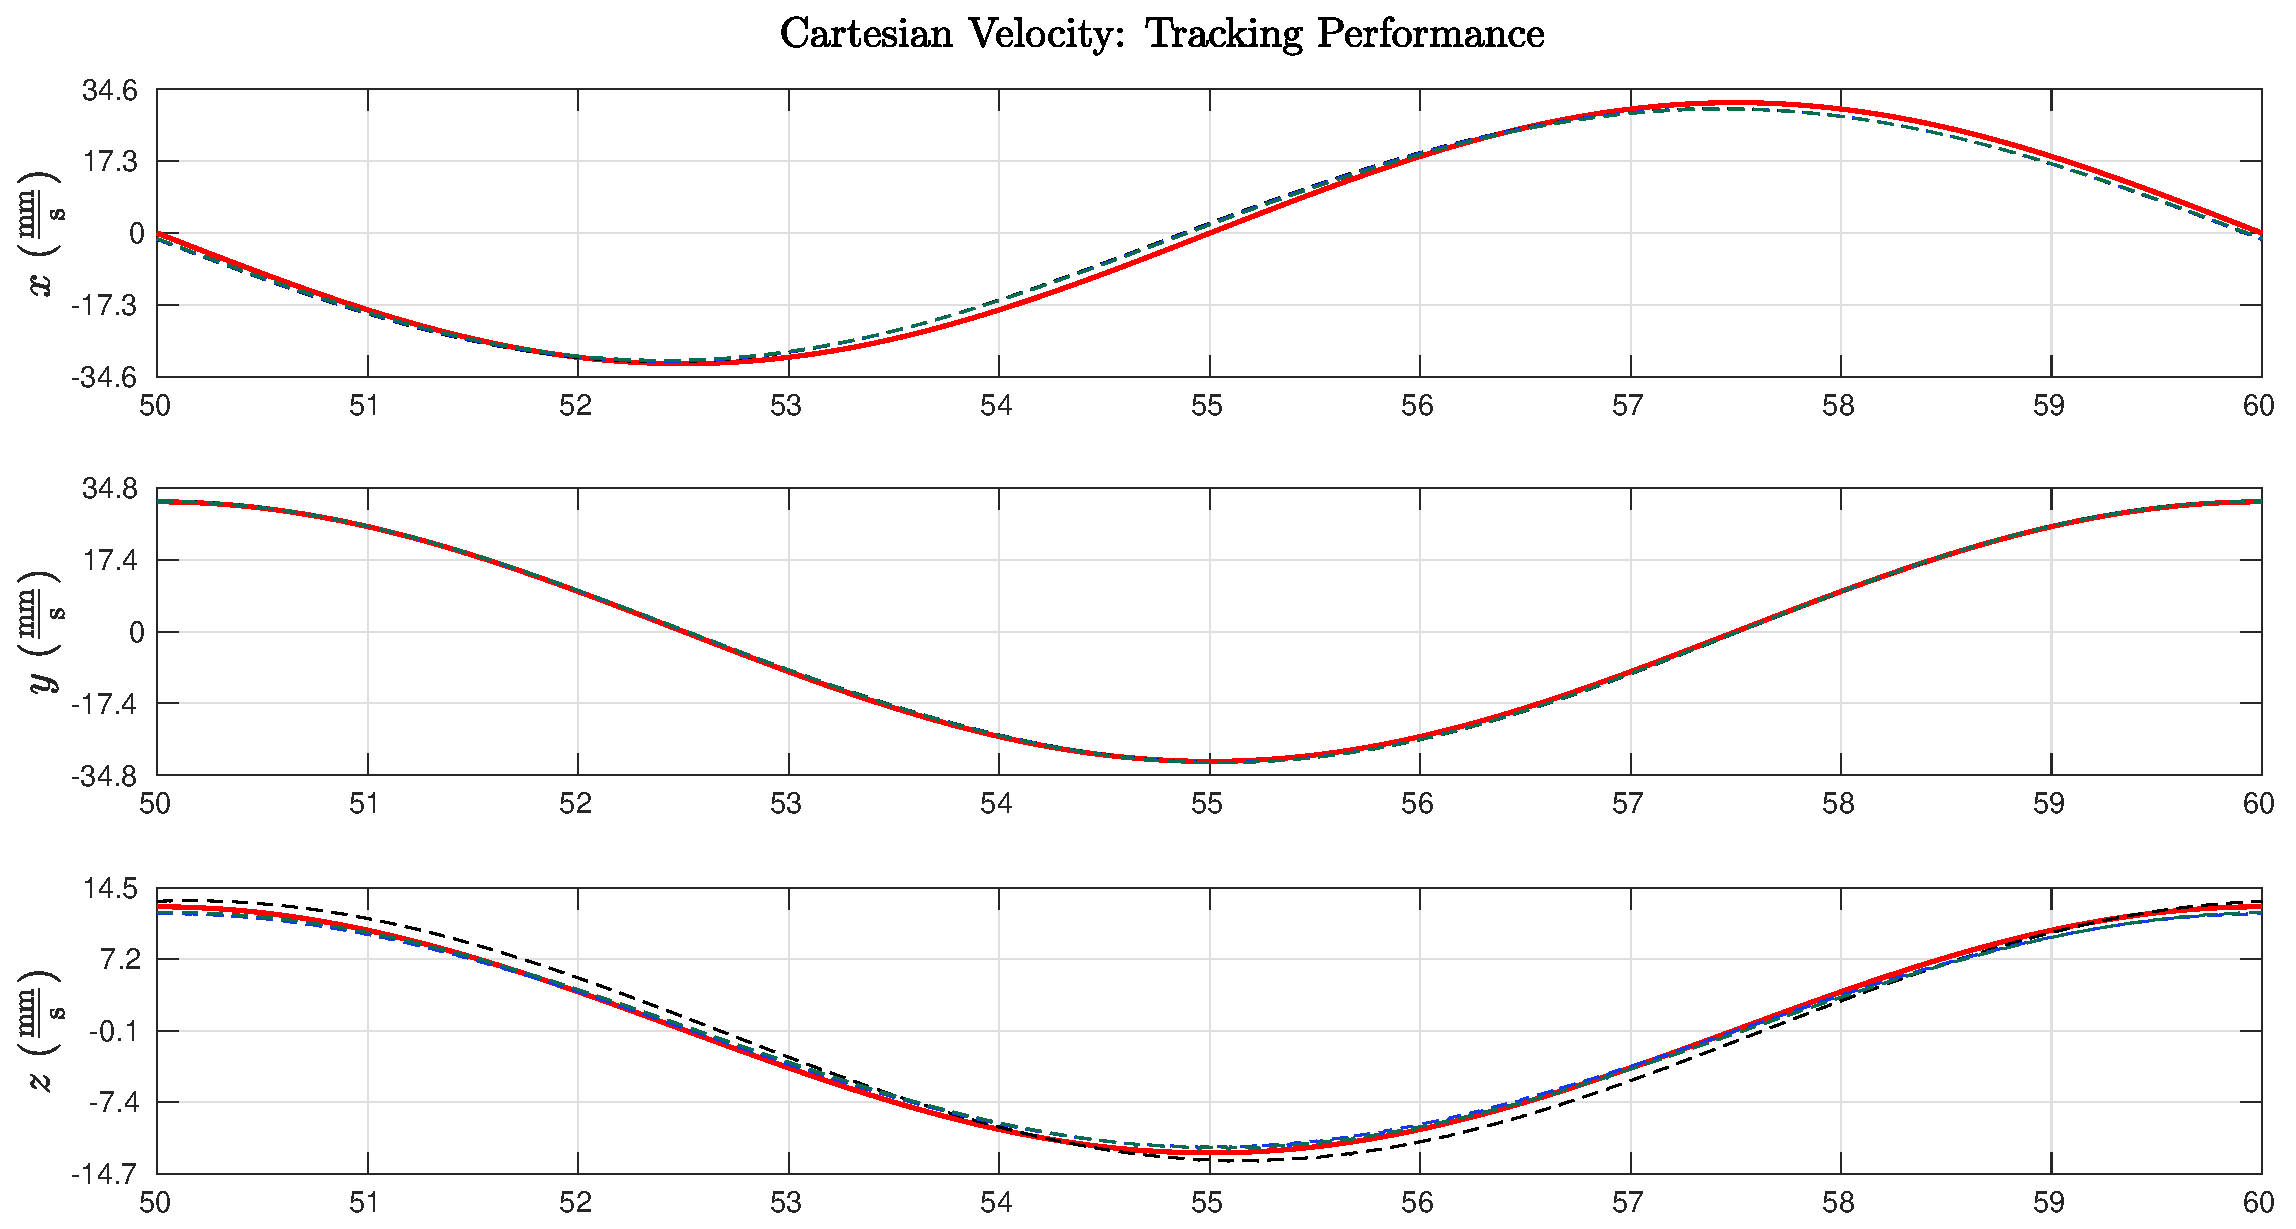
\includegraphics[width=1.1\textwidth]{img/SMCi/circular_traj/60_seg/articular_SMCi_vel_xyz_compare.eps}
		\end{figure}
	\end{frame}
	
	\begin{frame}[fragile]{Control de modo deslizante}
		\begin{figure}
			\centering
			\hspace*{-0.5cm}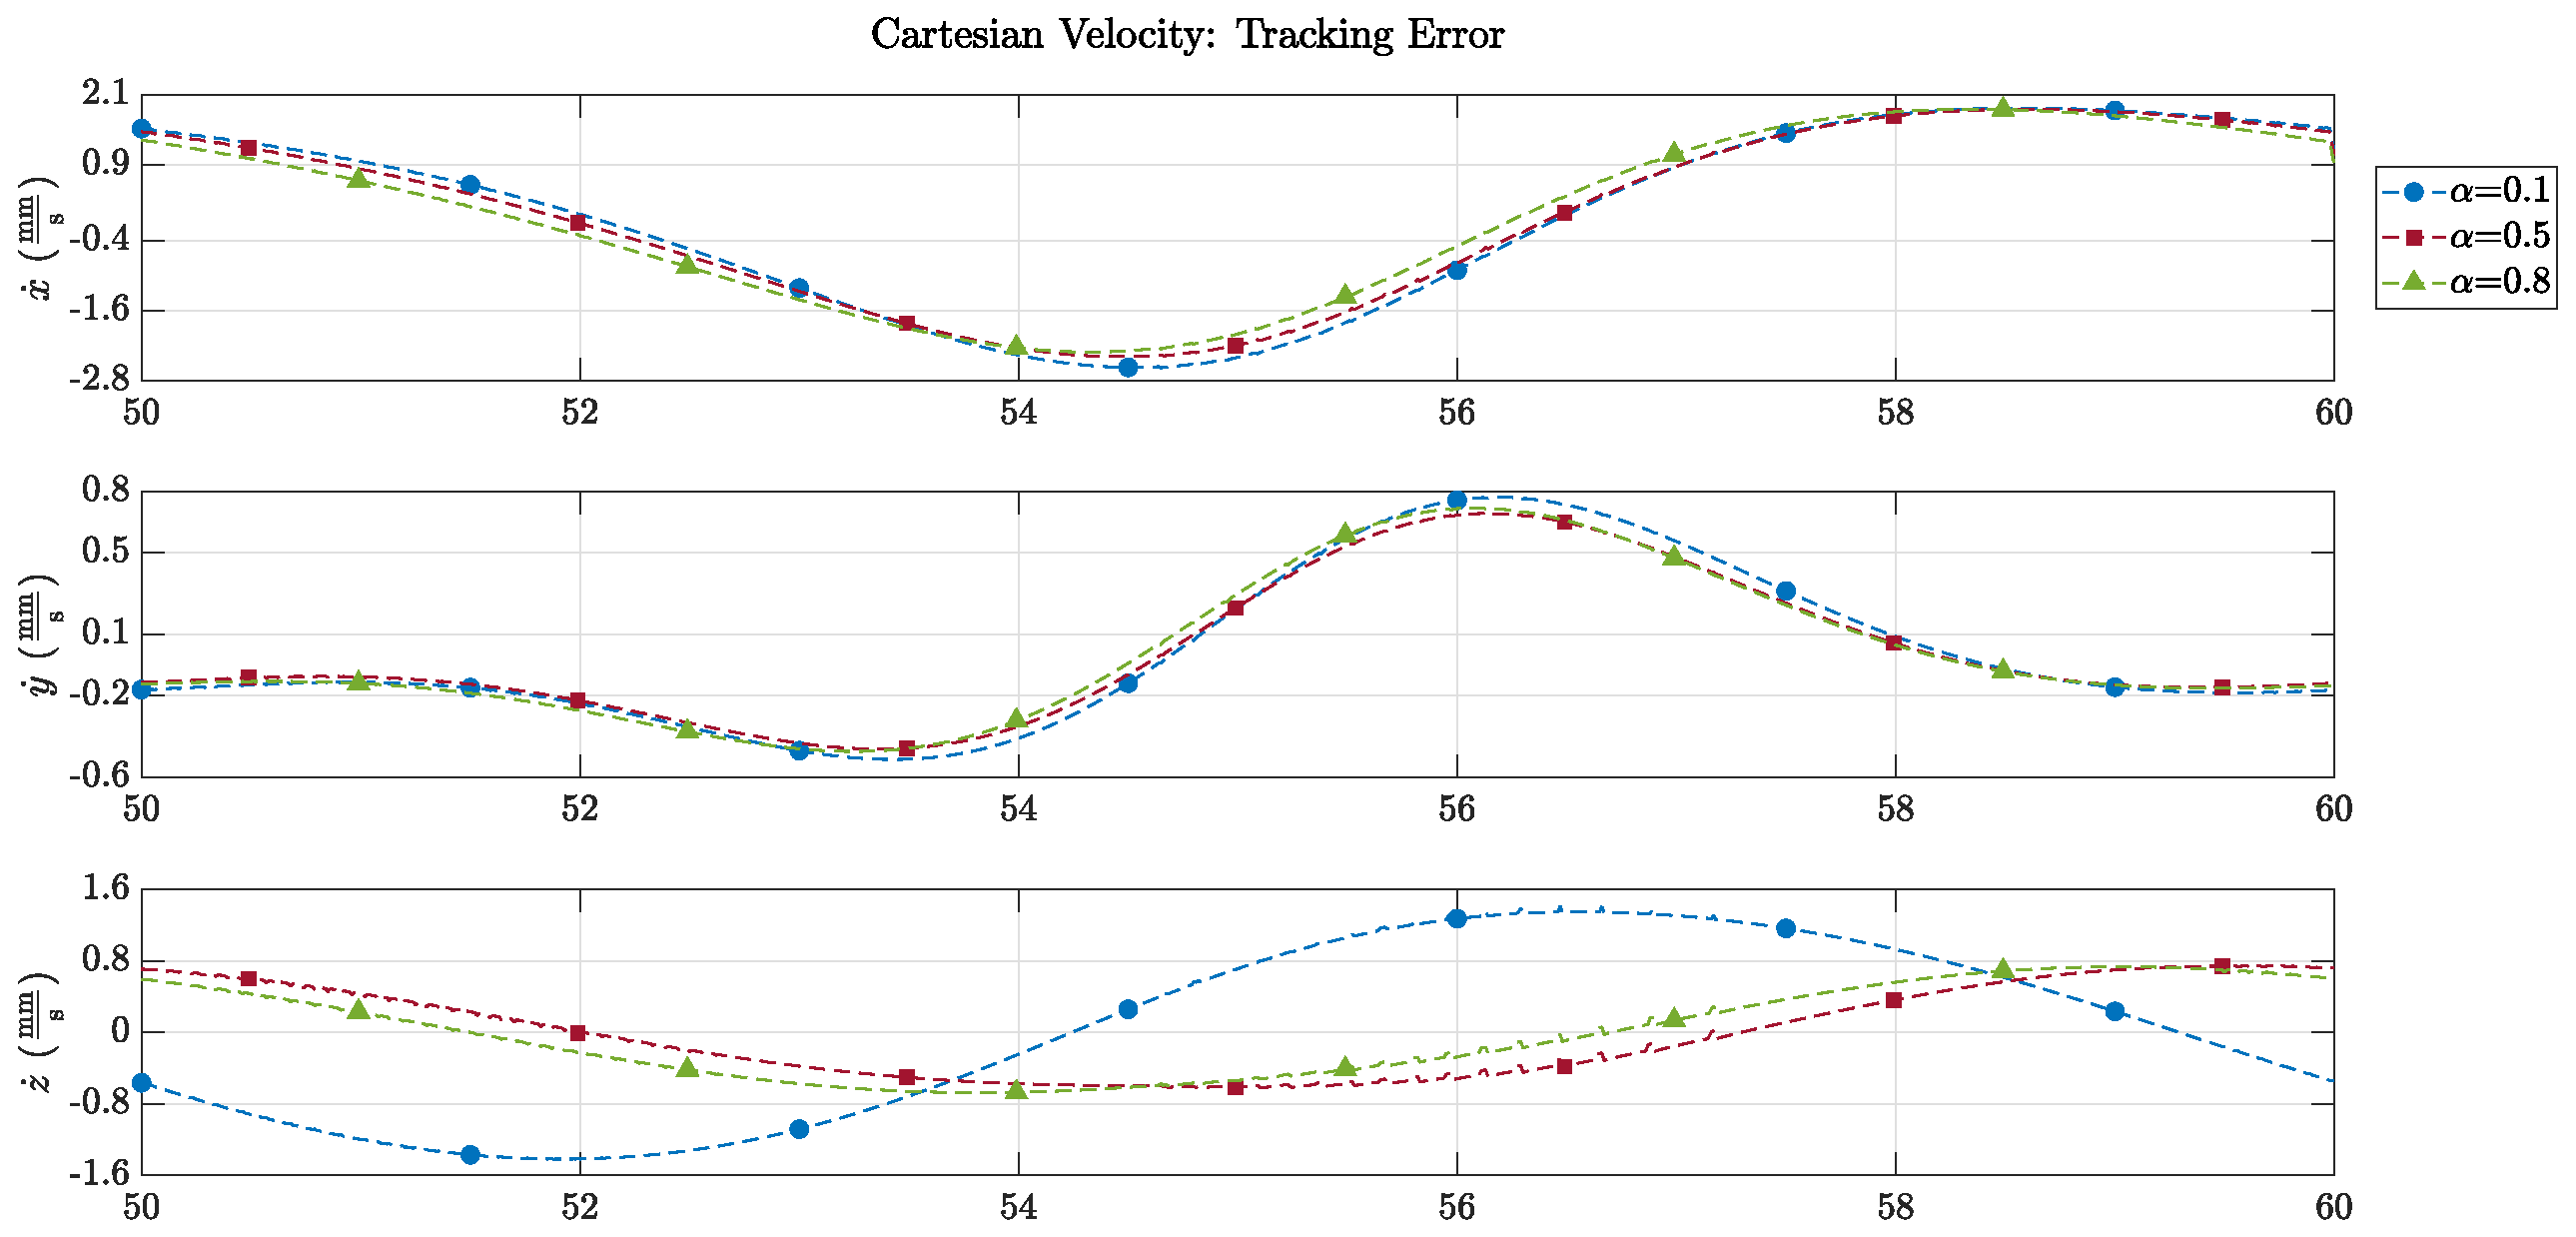
\includegraphics[width=1.1\textwidth]{img/SMCi/circular_traj/60_seg/articular_SMCi_vel_xyz_error_compare.eps}
		\end{figure}
	\end{frame}


	\begin{frame}[fragile]{Control de modo deslizante}
		\begin{figure}
			\centering
			\hspace*{-0.5cm}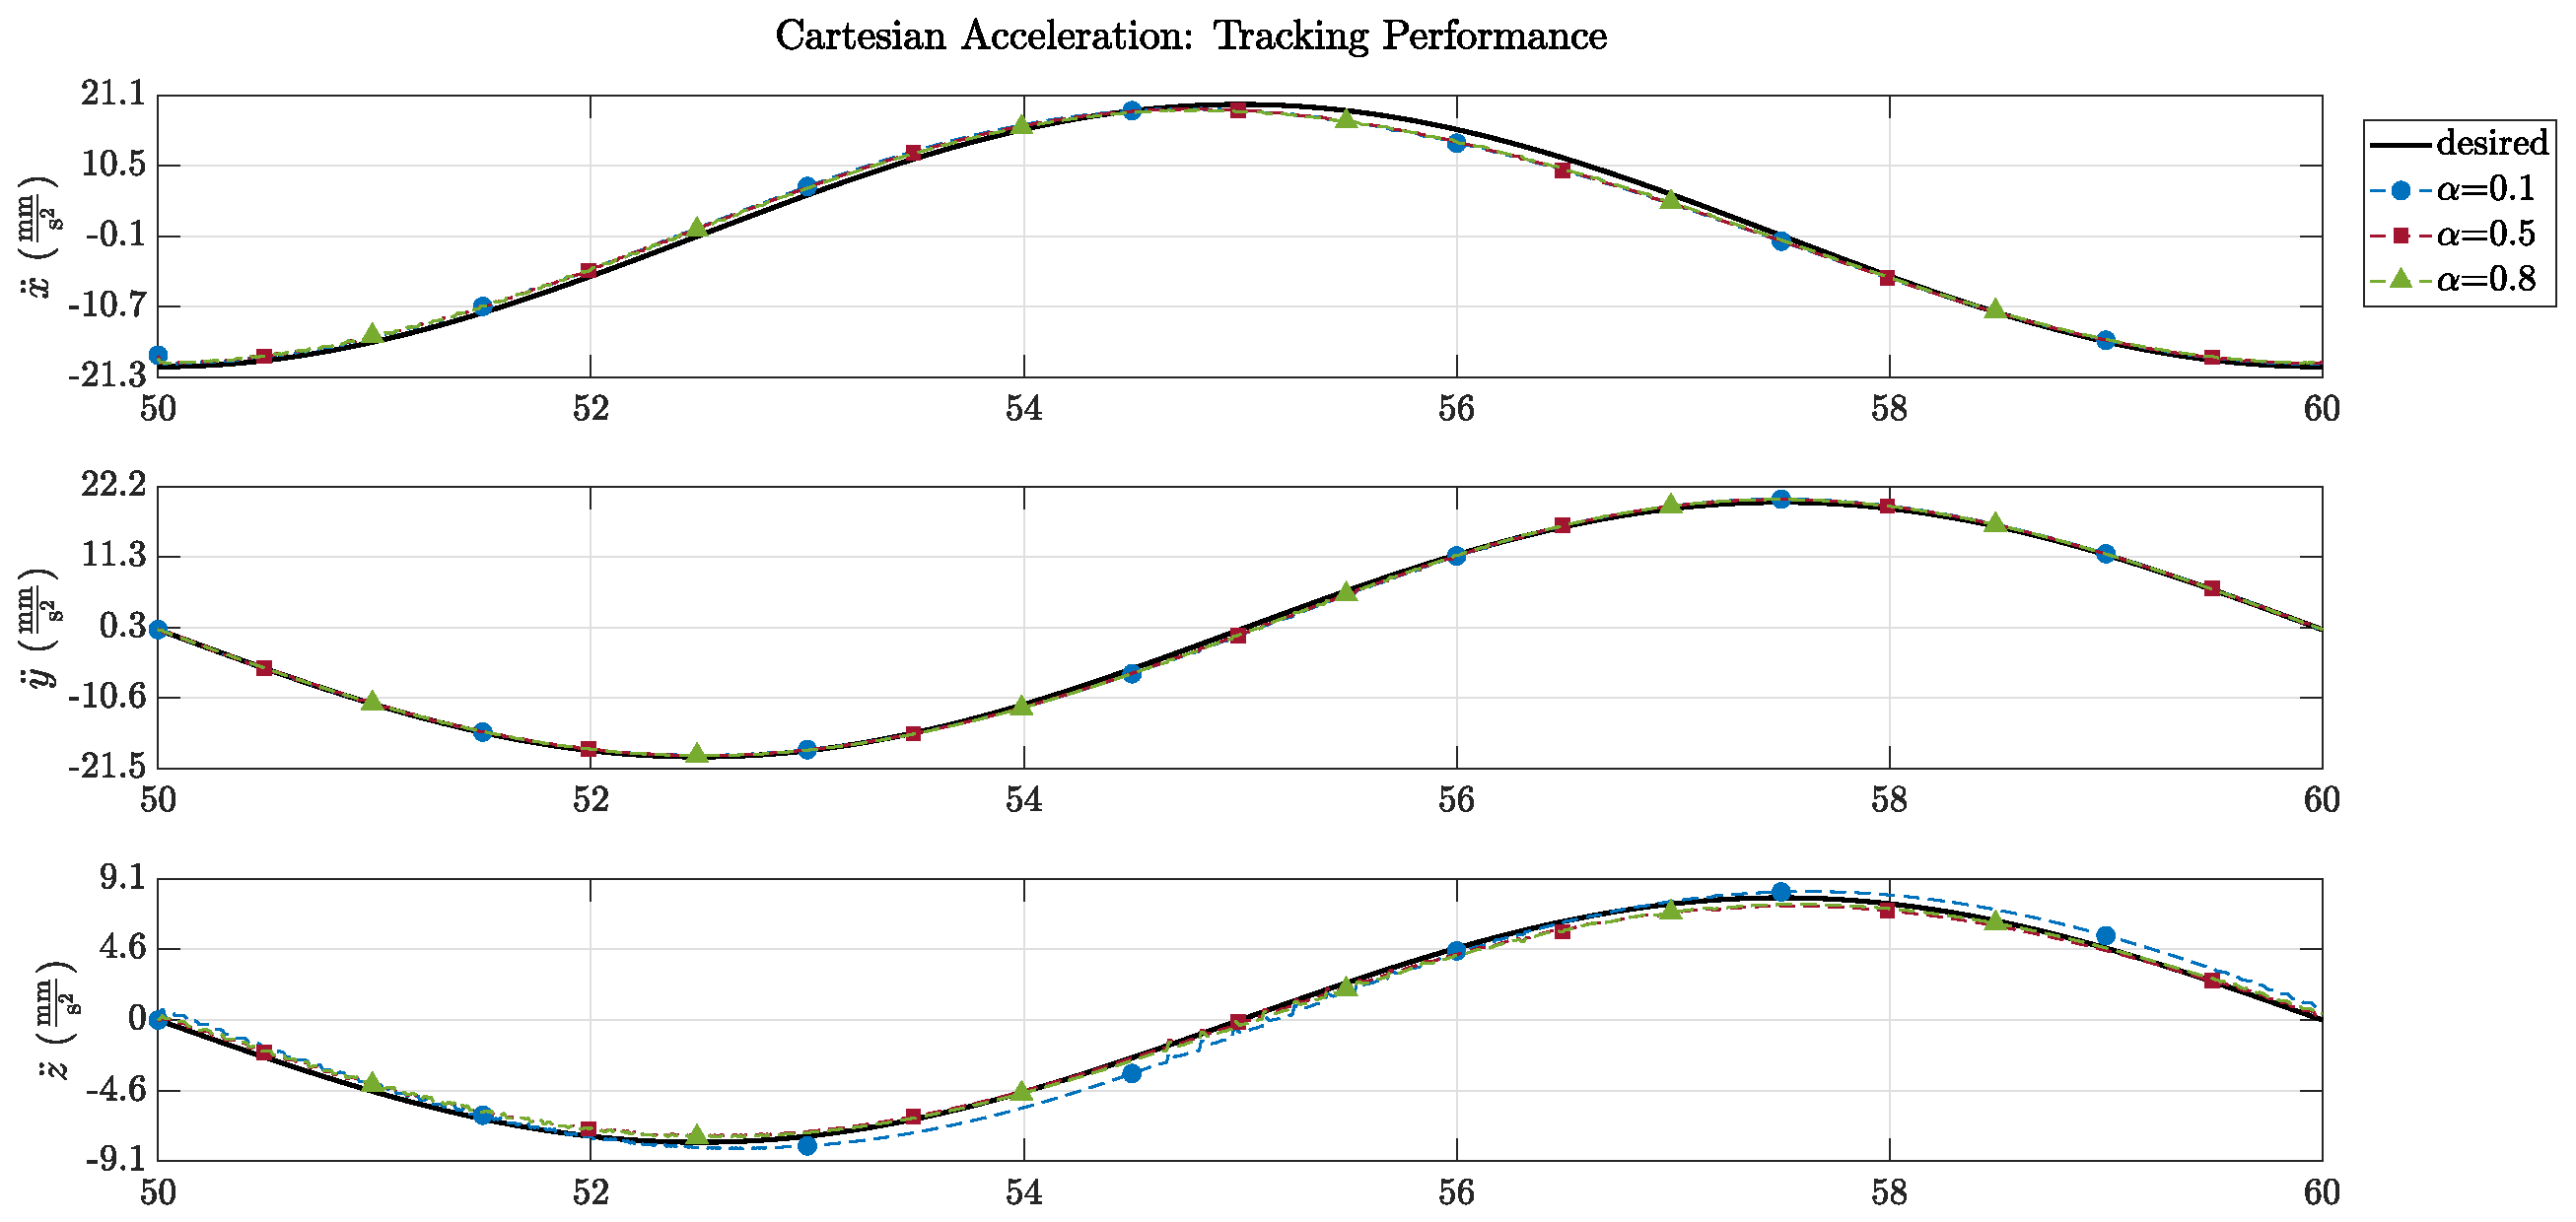
\includegraphics[width=1.1\textwidth]{img/SMCi/circular_traj/60_seg/articular_SMCi_accel_xyz_compare.eps}
		\end{figure}
	\end{frame}
	
	\begin{frame}[fragile]{Control de modo deslizante}
		\begin{figure}
			\centering
			\hspace*{-0.5cm}\includegraphics[width=1.1\textwidth]{img/SMCi/circular_traj/60_seg/articular_SMCi_accel_xyz_error_compare.eps}
		\end{figure}
	\end{frame}

	\begin{frame}[fragile]{Control de modo deslizante}
		\begin{figure}
			\centering
			\hspace*{-0.5cm}\includegraphics[width=1.1\textwidth]{img/SMCi/circular_traj/60_seg/articular_SMCi_jerk_xyz_compare.eps}
		\end{figure}
	\end{frame}
	
	\begin{frame}[fragile]{Control de modo deslizante}
		\begin{figure}
			\centering
			\hspace*{-0.5cm}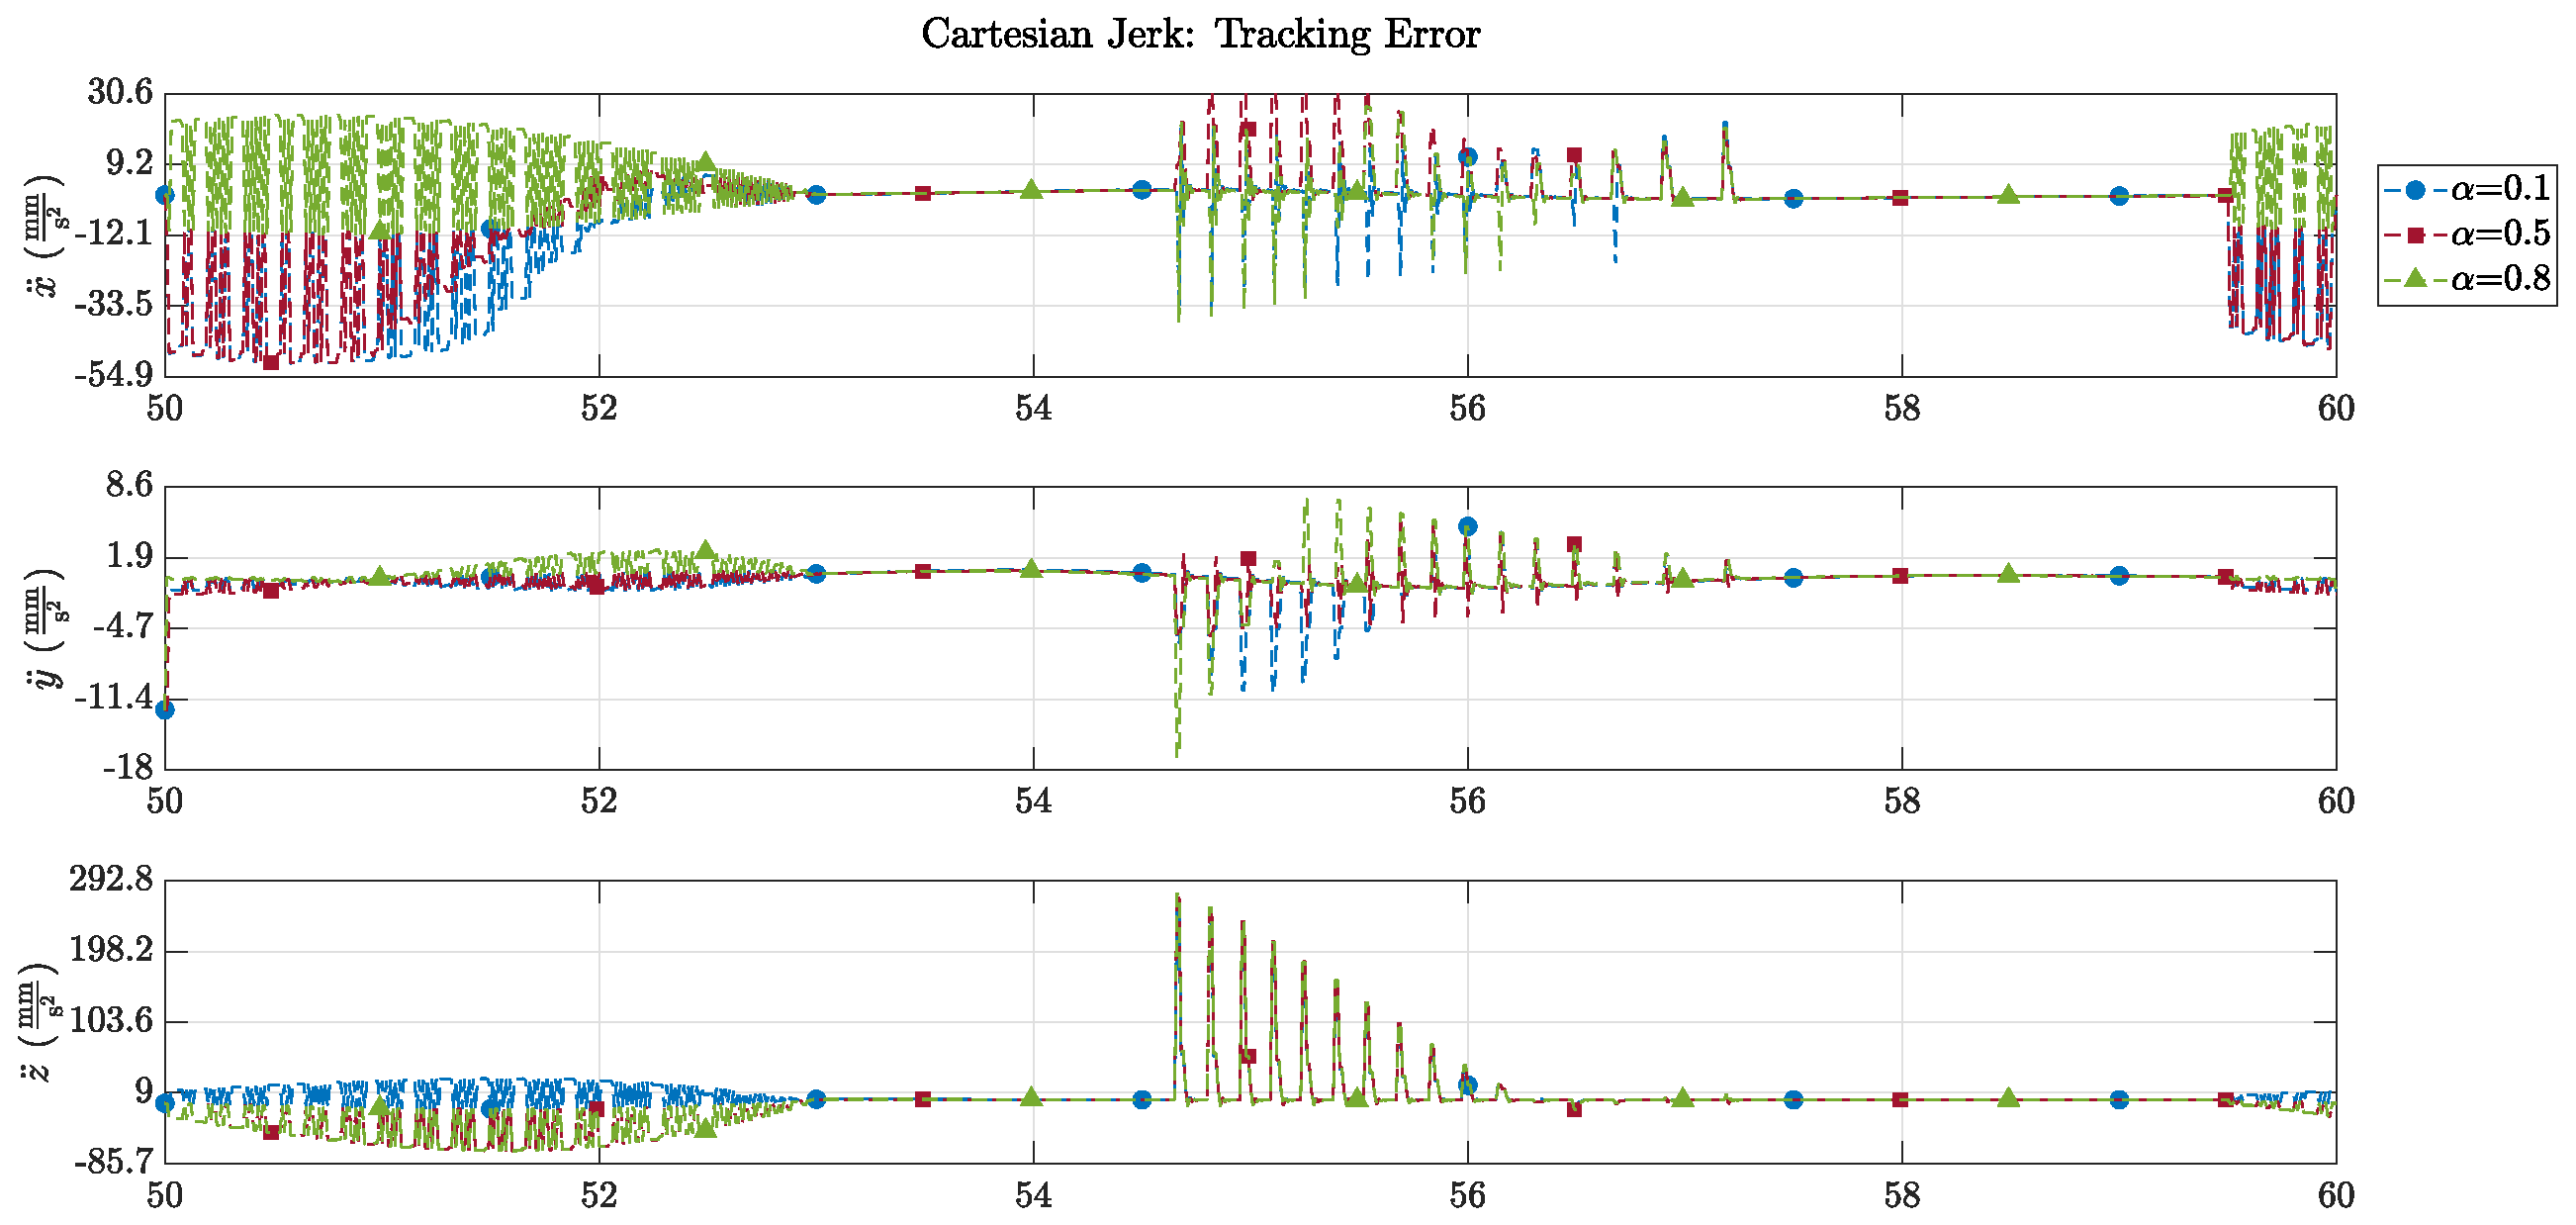
\includegraphics[width=1.1\textwidth]{img/SMCi/circular_traj/60_seg/articular_SMCi_jerk_xyz_error_compare.eps}
		\end{figure}
	\end{frame}
	
	\begin{frame}[fragile]{Control de modo deslizante}
		\begin{figure}
			\centering
			\hspace*{-0.5cm}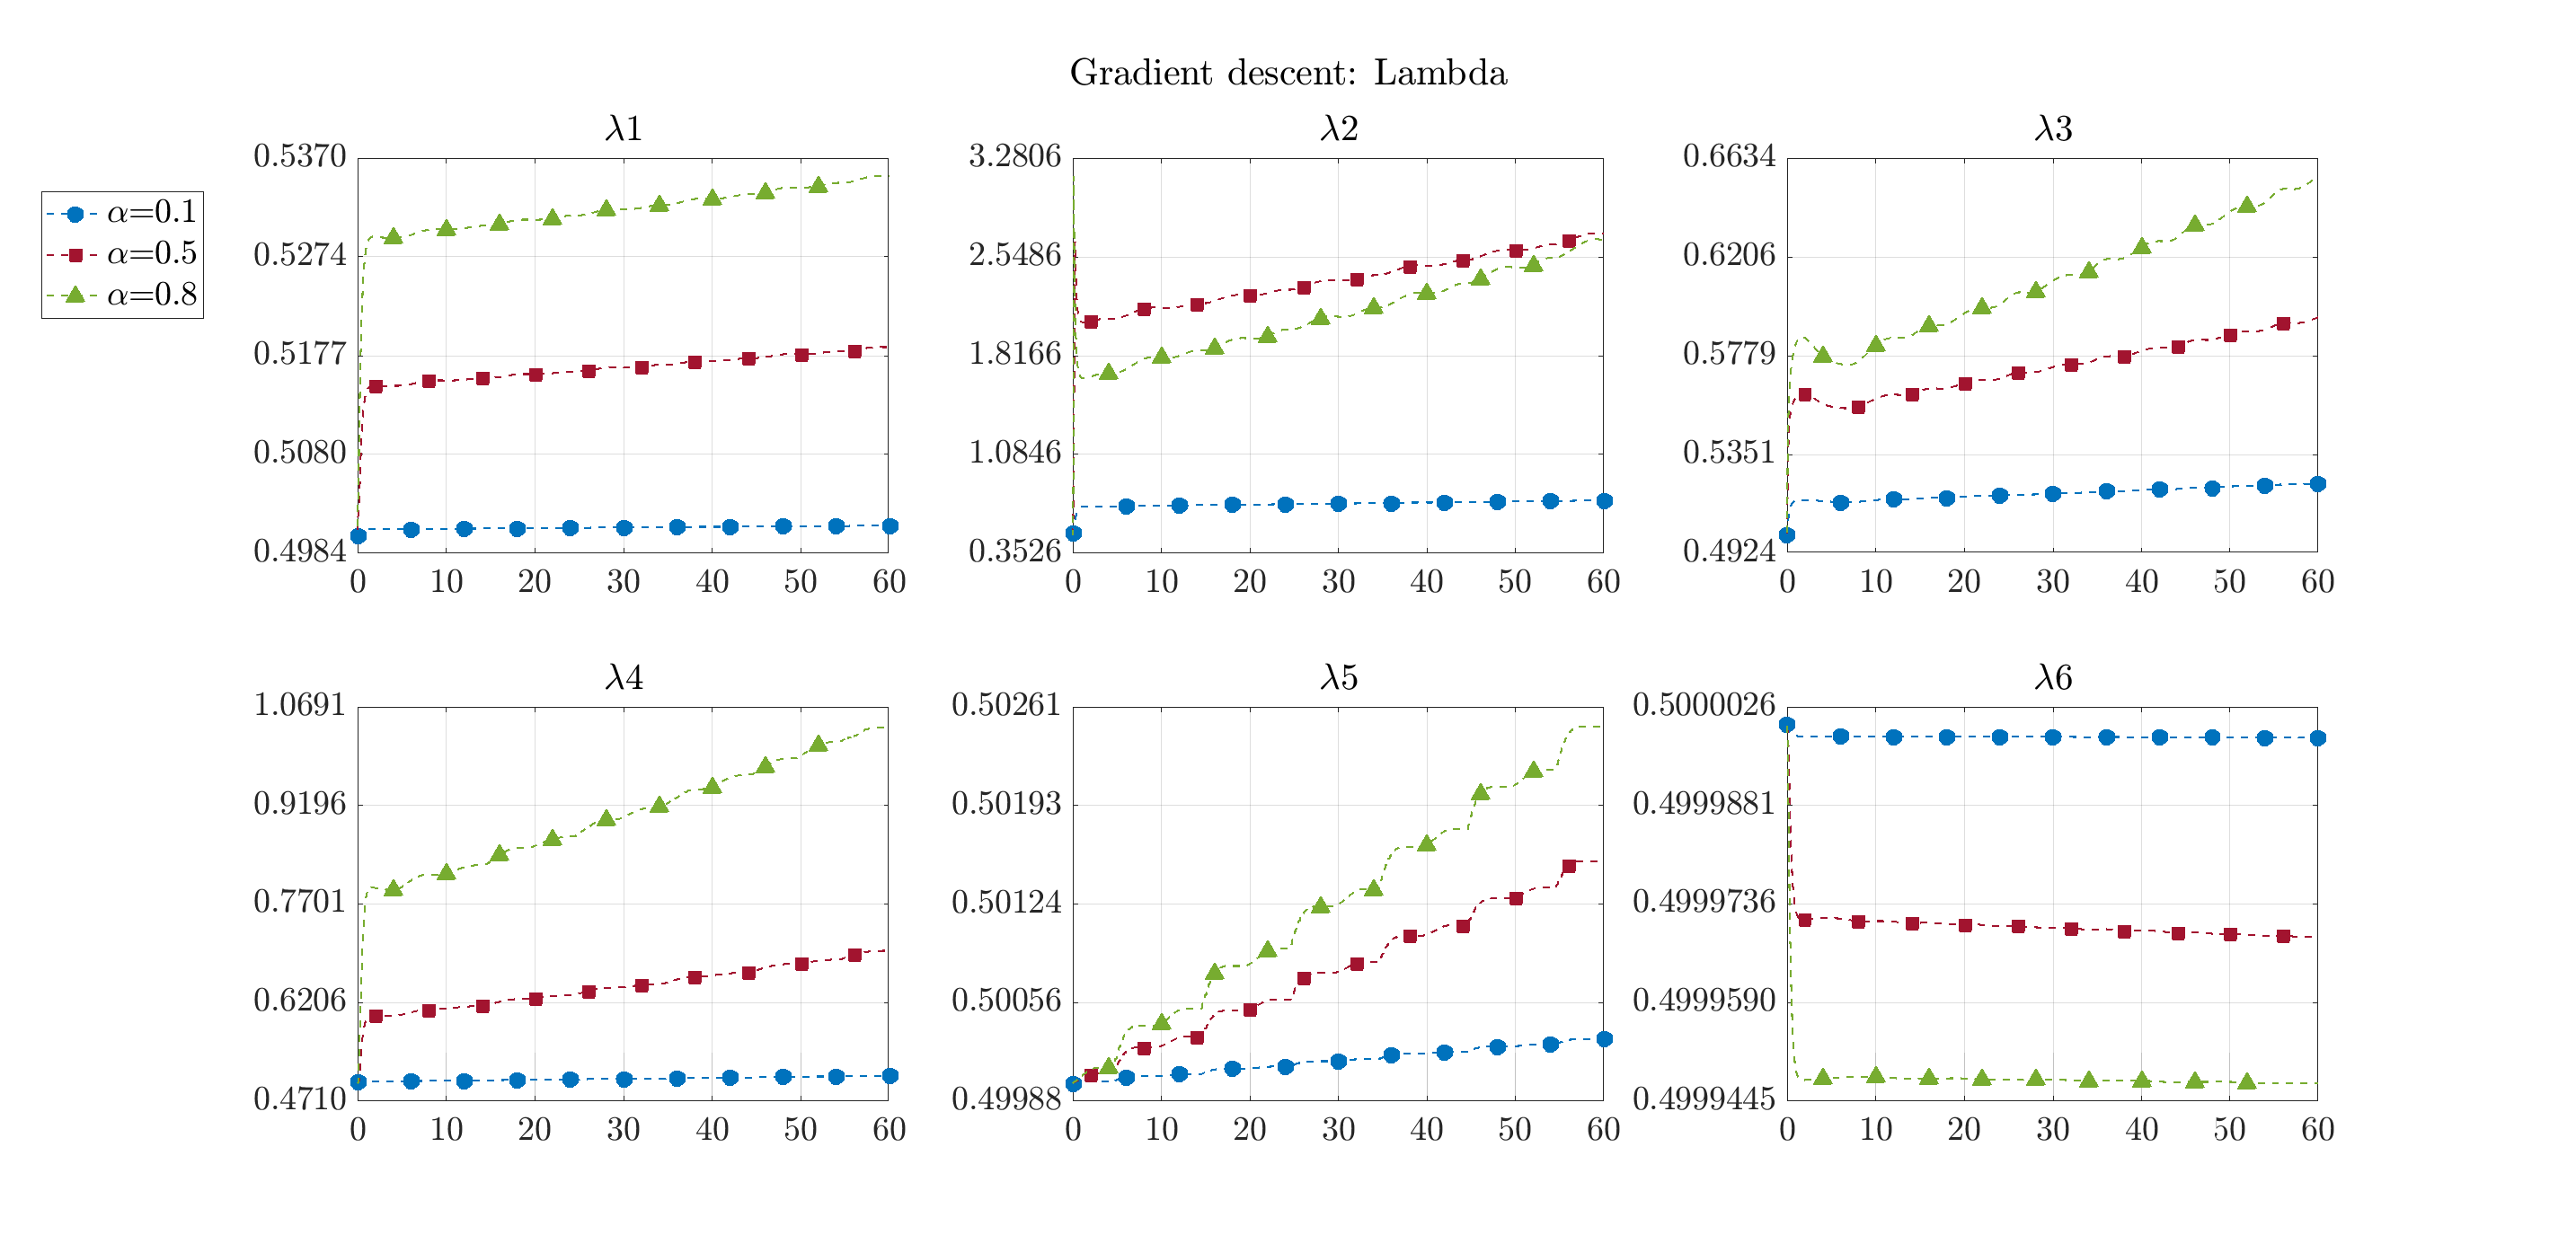
\includegraphics[width=1.1\textwidth]{img/SMCi/circular_traj/60_seg/articular_SMCi_lambda_compare.eps}
		\end{figure}
	\end{frame}
	
	
	
	\begin{frame}[fragile]{Parámetros de la segunda simulación ($600$ segundos)}
		\begin{minipage}{\textwidth}
			\large \color{darkblue}{\textbf{Datos del controlador}} 
			\begin{itemize}
				\item Se realizan simulaciones para: $\alpha=0.1$, $0.5$, $0.8$.
				
				\item Se mantiene constante: $\gamma=0.999$ y $\beta=0.001$.
				
				\item La ganancia de control se inicia con: $\lambda=0.5$.
			\end{itemize}
			\color{white}{para crear espacio, borrar luego}	 
		\end{minipage}
		
		\begin{minipage}{\textwidth}		
			\large \color{darkblue}{\textbf{Datos de la trayectoria}}
			\begin{itemize}
				\item Trayectoria circular de radio $0.5$ m en el plano XY.
				
				\item Trayectoria sinusoidal de amplitud $0.2$ m en el eje Z.
				
				\item El periodo de las trayectorias es $10$ segundos.
			\end{itemize}
		\end{minipage}		
	\end{frame}	
	
	
	
	\begin{frame}[fragile]{Control de modo deslizante}
		\begin{figure}
			\centering
			\hspace*{-0.7cm}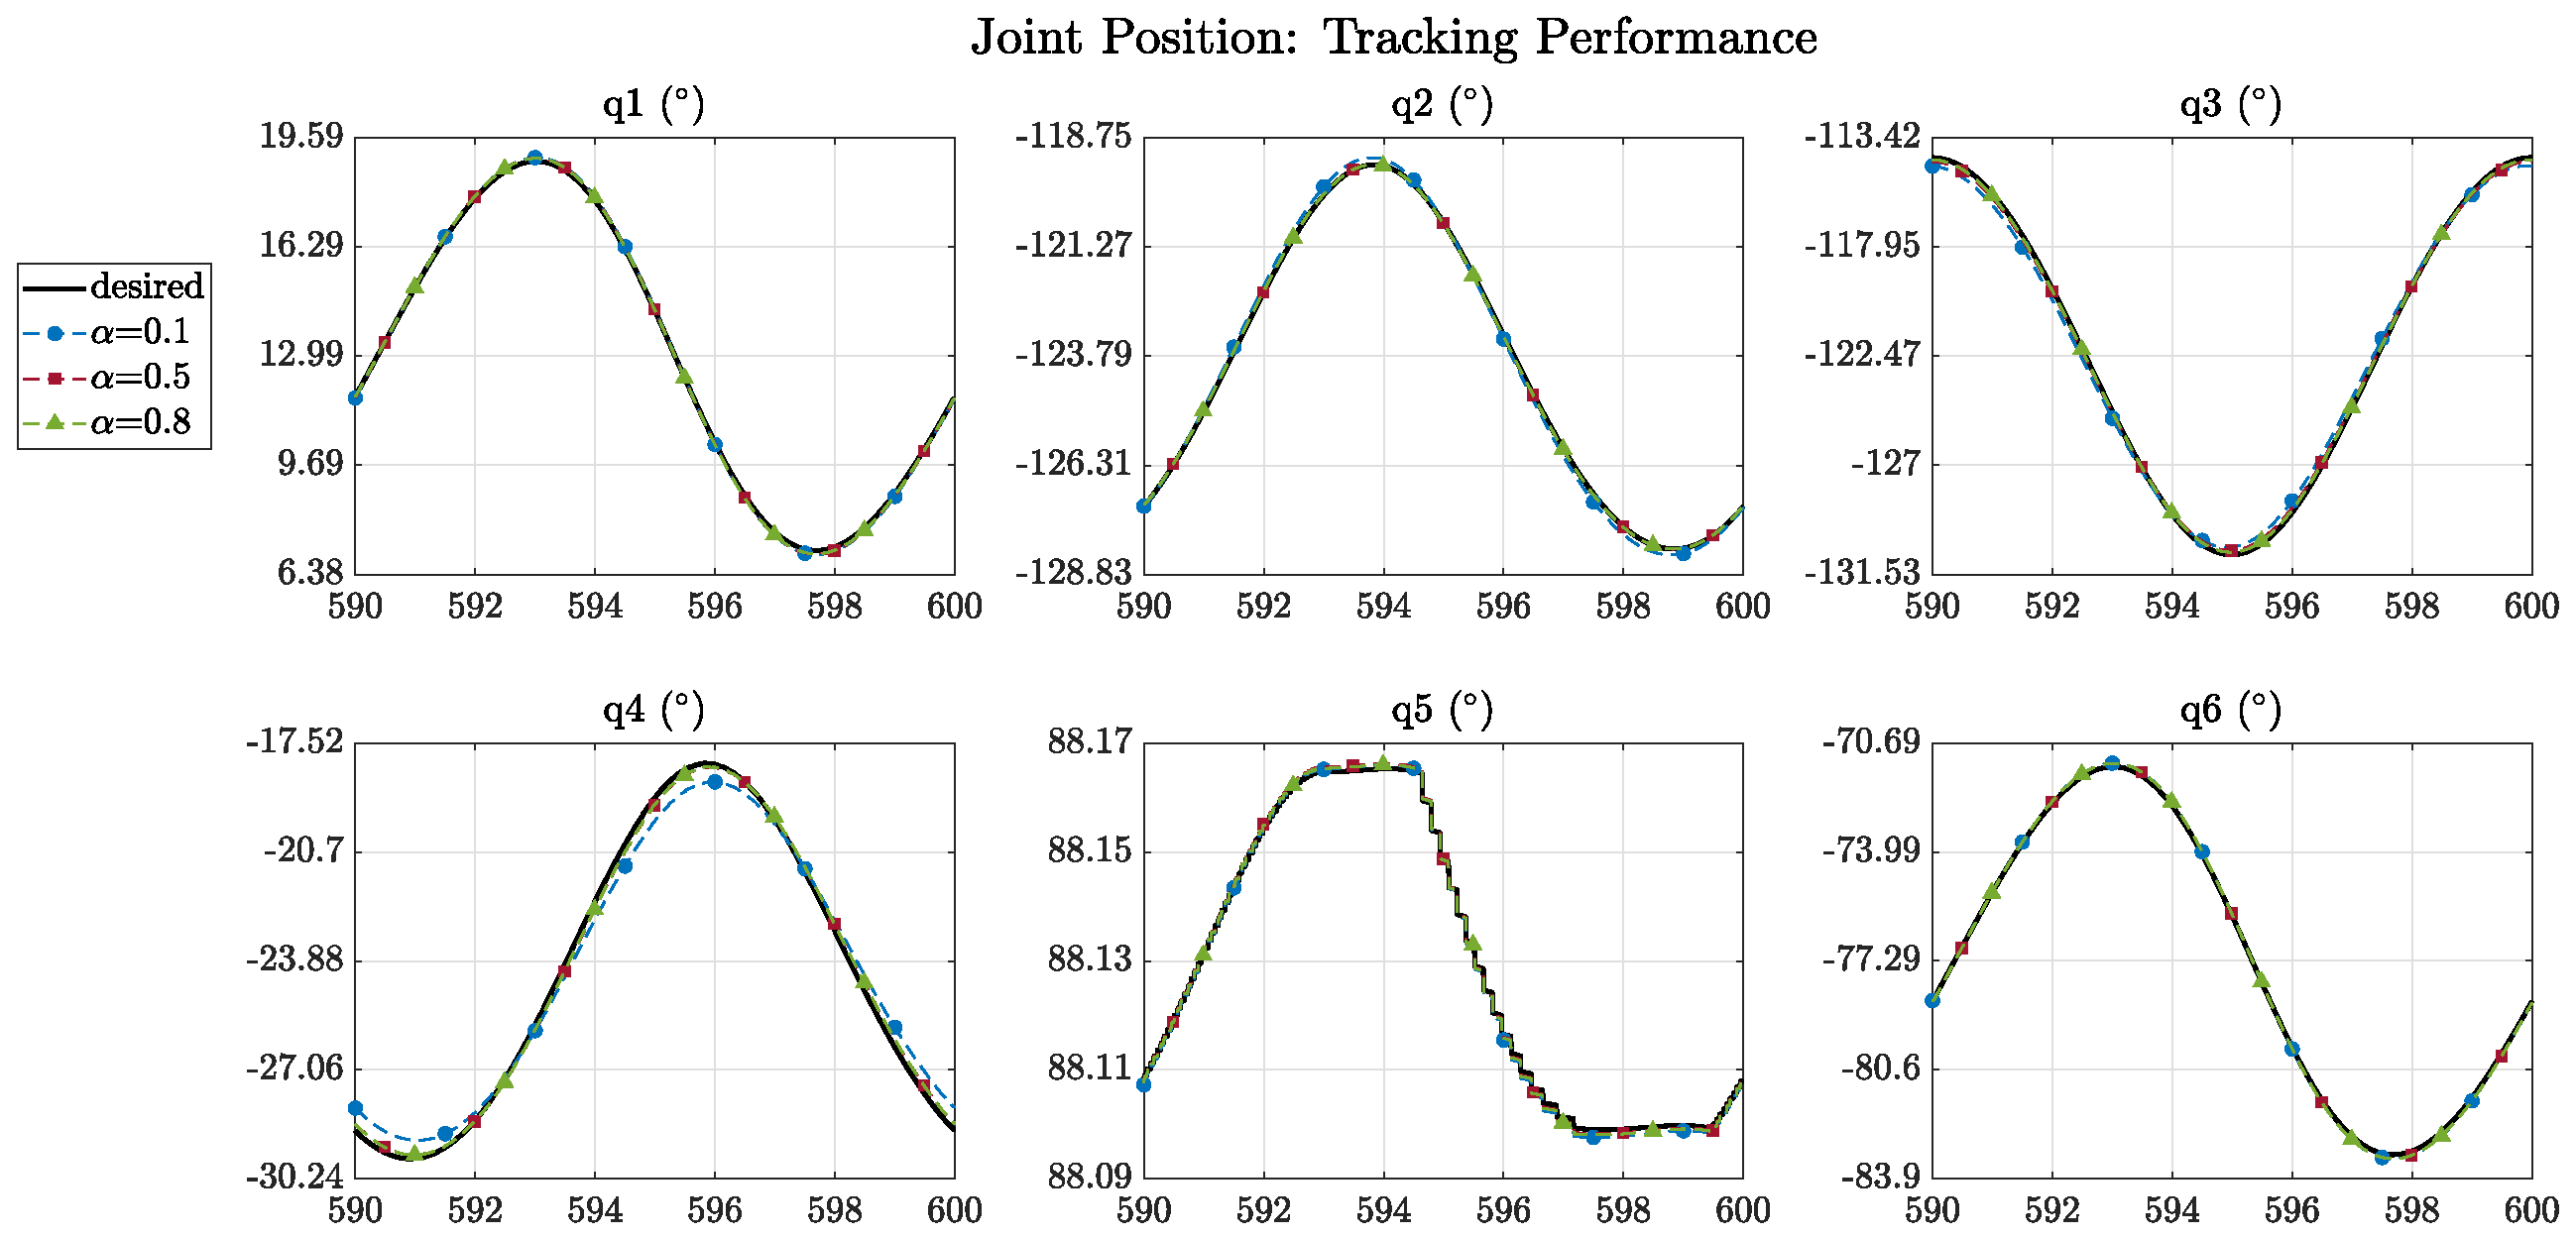
\includegraphics[width=1.1\textwidth]{img/SMCi/circular_traj/600_seg/articular_SMCi_position_compare.eps}
		\end{figure}
	\end{frame}
	
	\begin{frame}[fragile]{Control de modo deslizante}
		\begin{figure}
			\centering
			\hspace*{-0.7cm}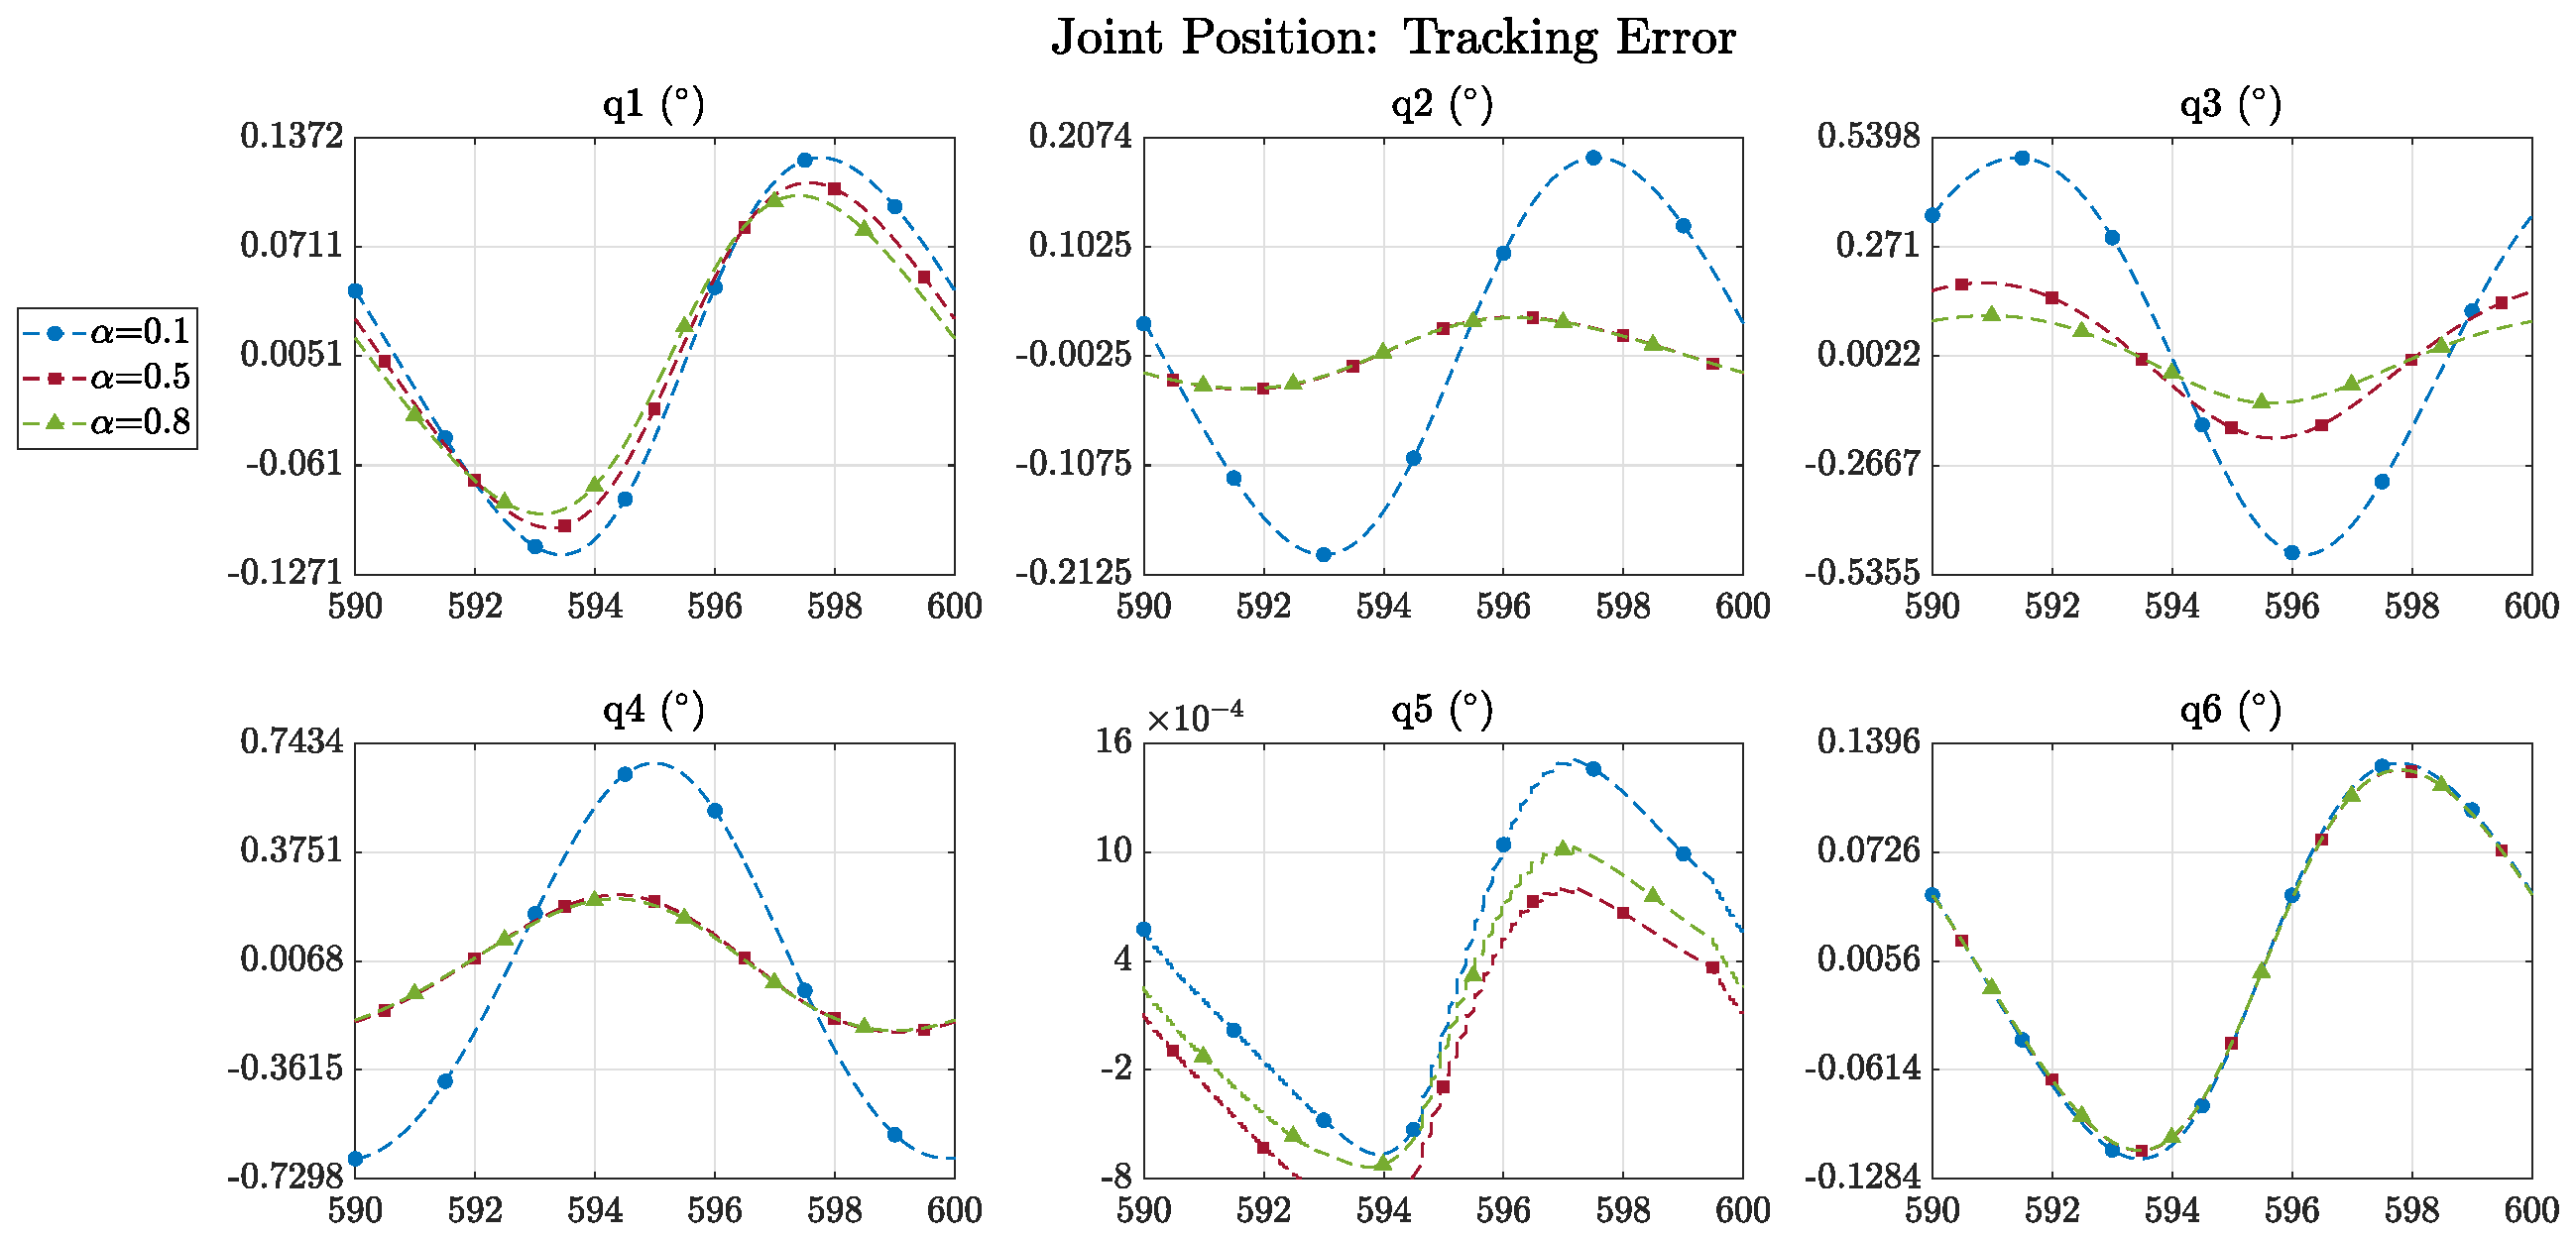
\includegraphics[width=1.1\textwidth]{img/SMCi/circular_traj/600_seg/articular_SMCi_position_error_compare.eps}
		\end{figure}
	\end{frame}	
	
	\begin{frame}[fragile]{Control de modo deslizante}
		\begin{figure}
			\centering
			\hspace*{-0.7cm}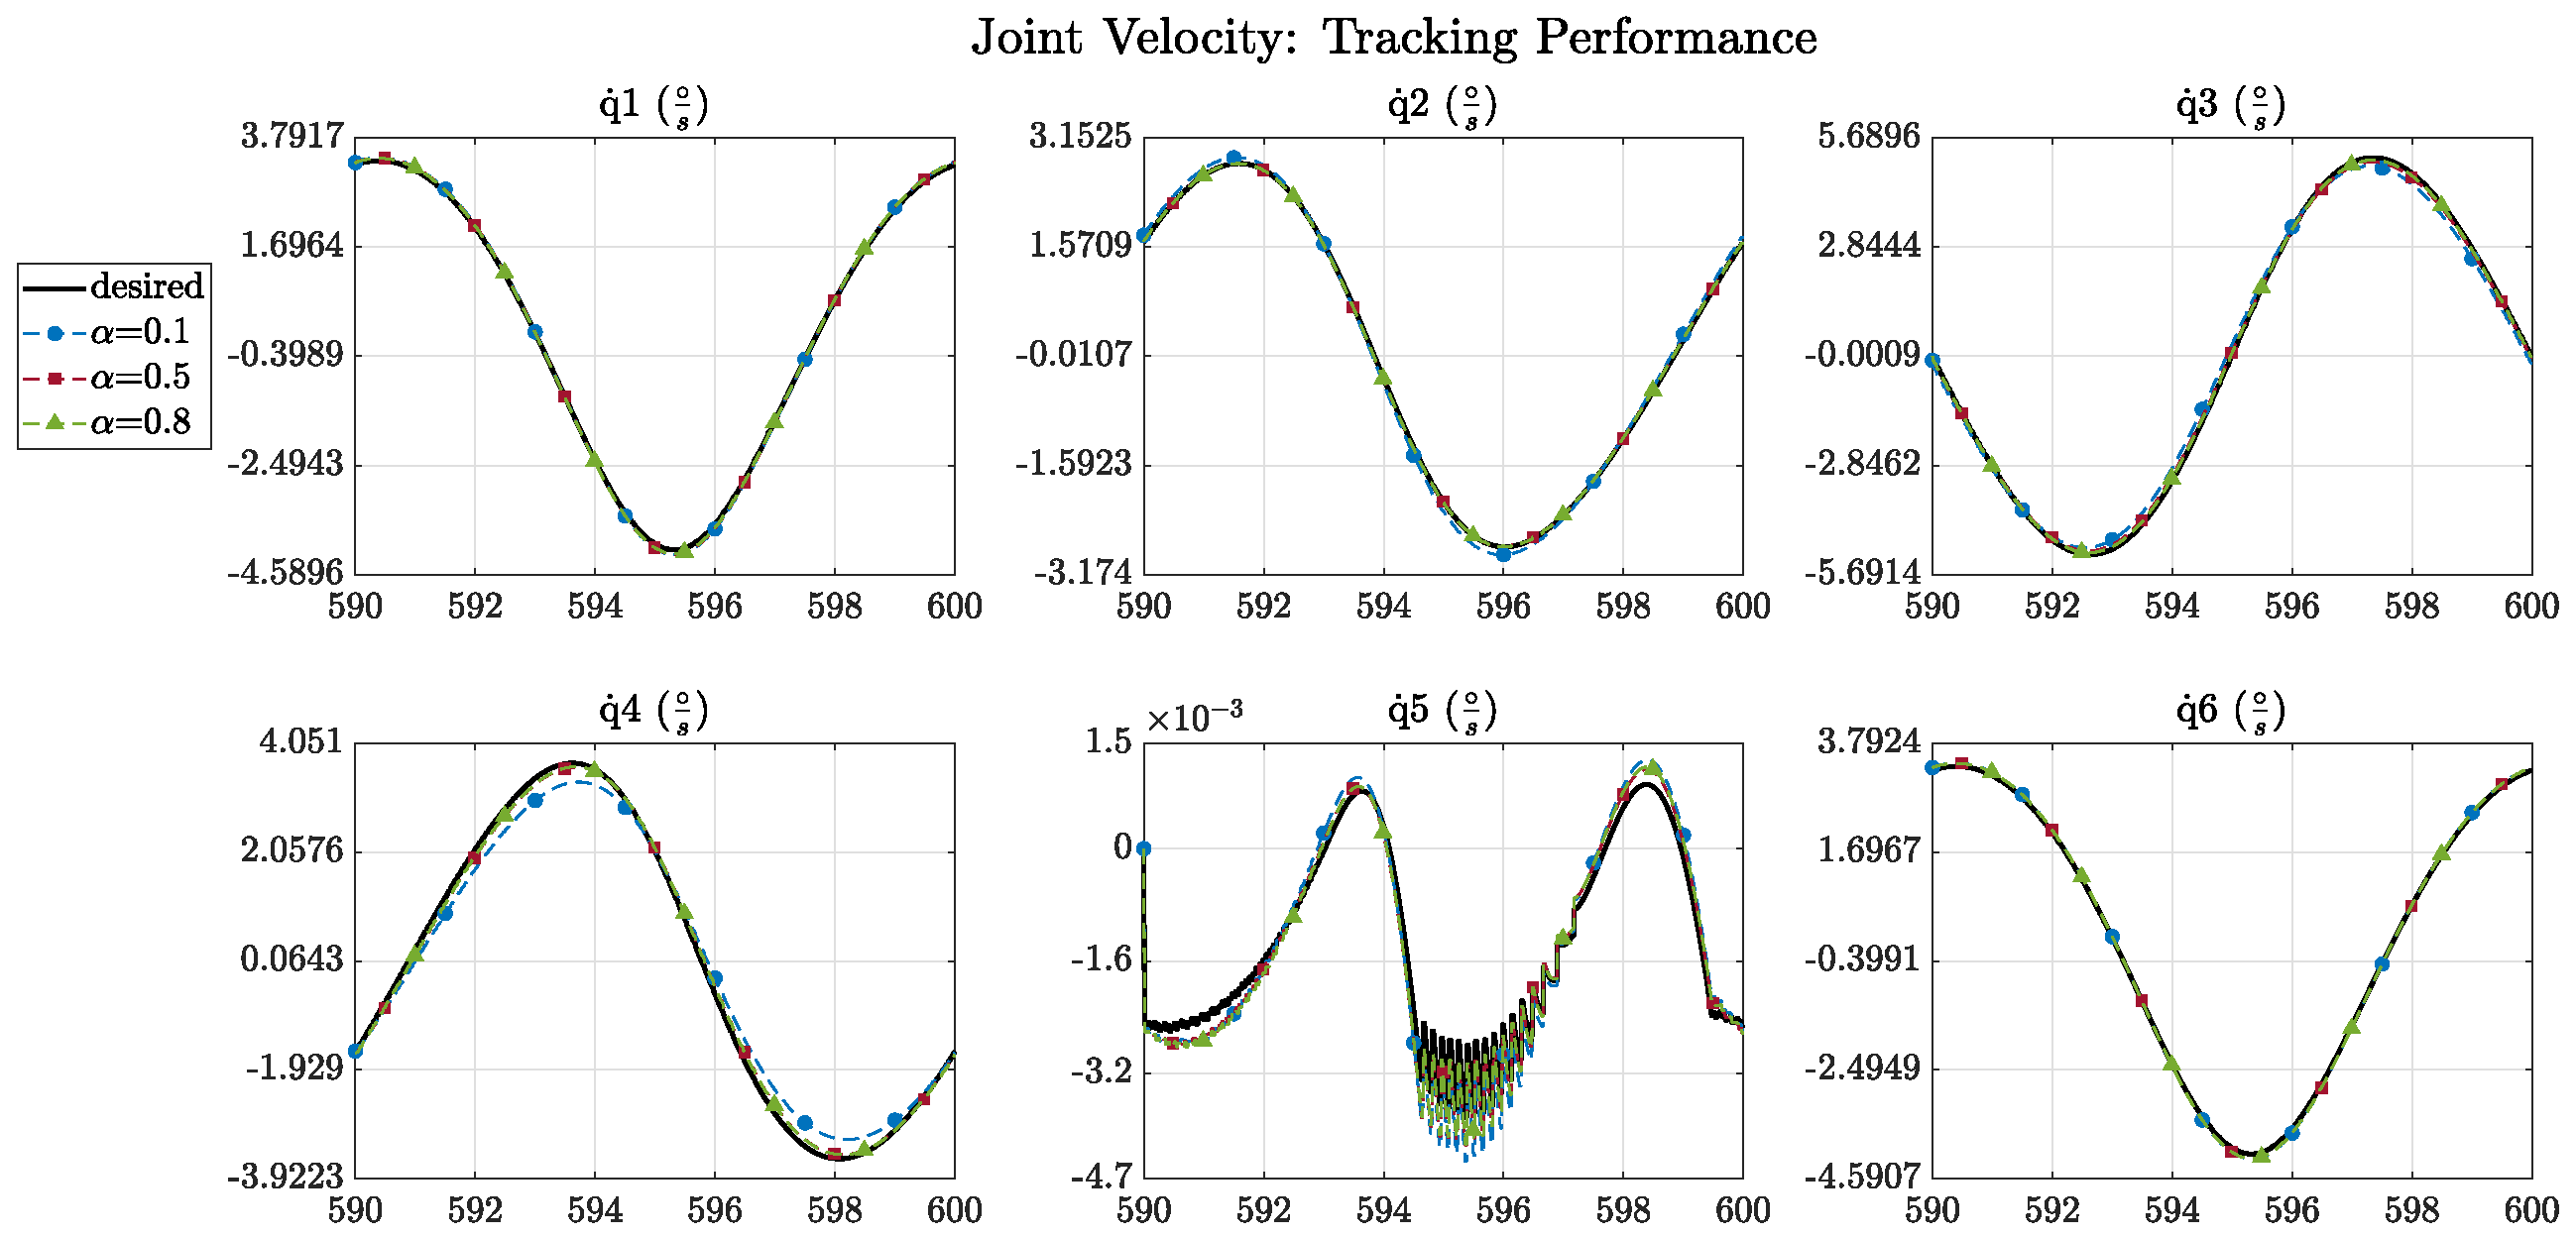
\includegraphics[width=1.1\textwidth]{img/SMCi/circular_traj/600_seg/articular_SMCi_velocity_compare.eps}
		\end{figure}
	\end{frame}
	
	\begin{frame}[fragile]{Control de modo deslizante}
		\begin{figure}
			\centering
			\hspace*{-0.7cm}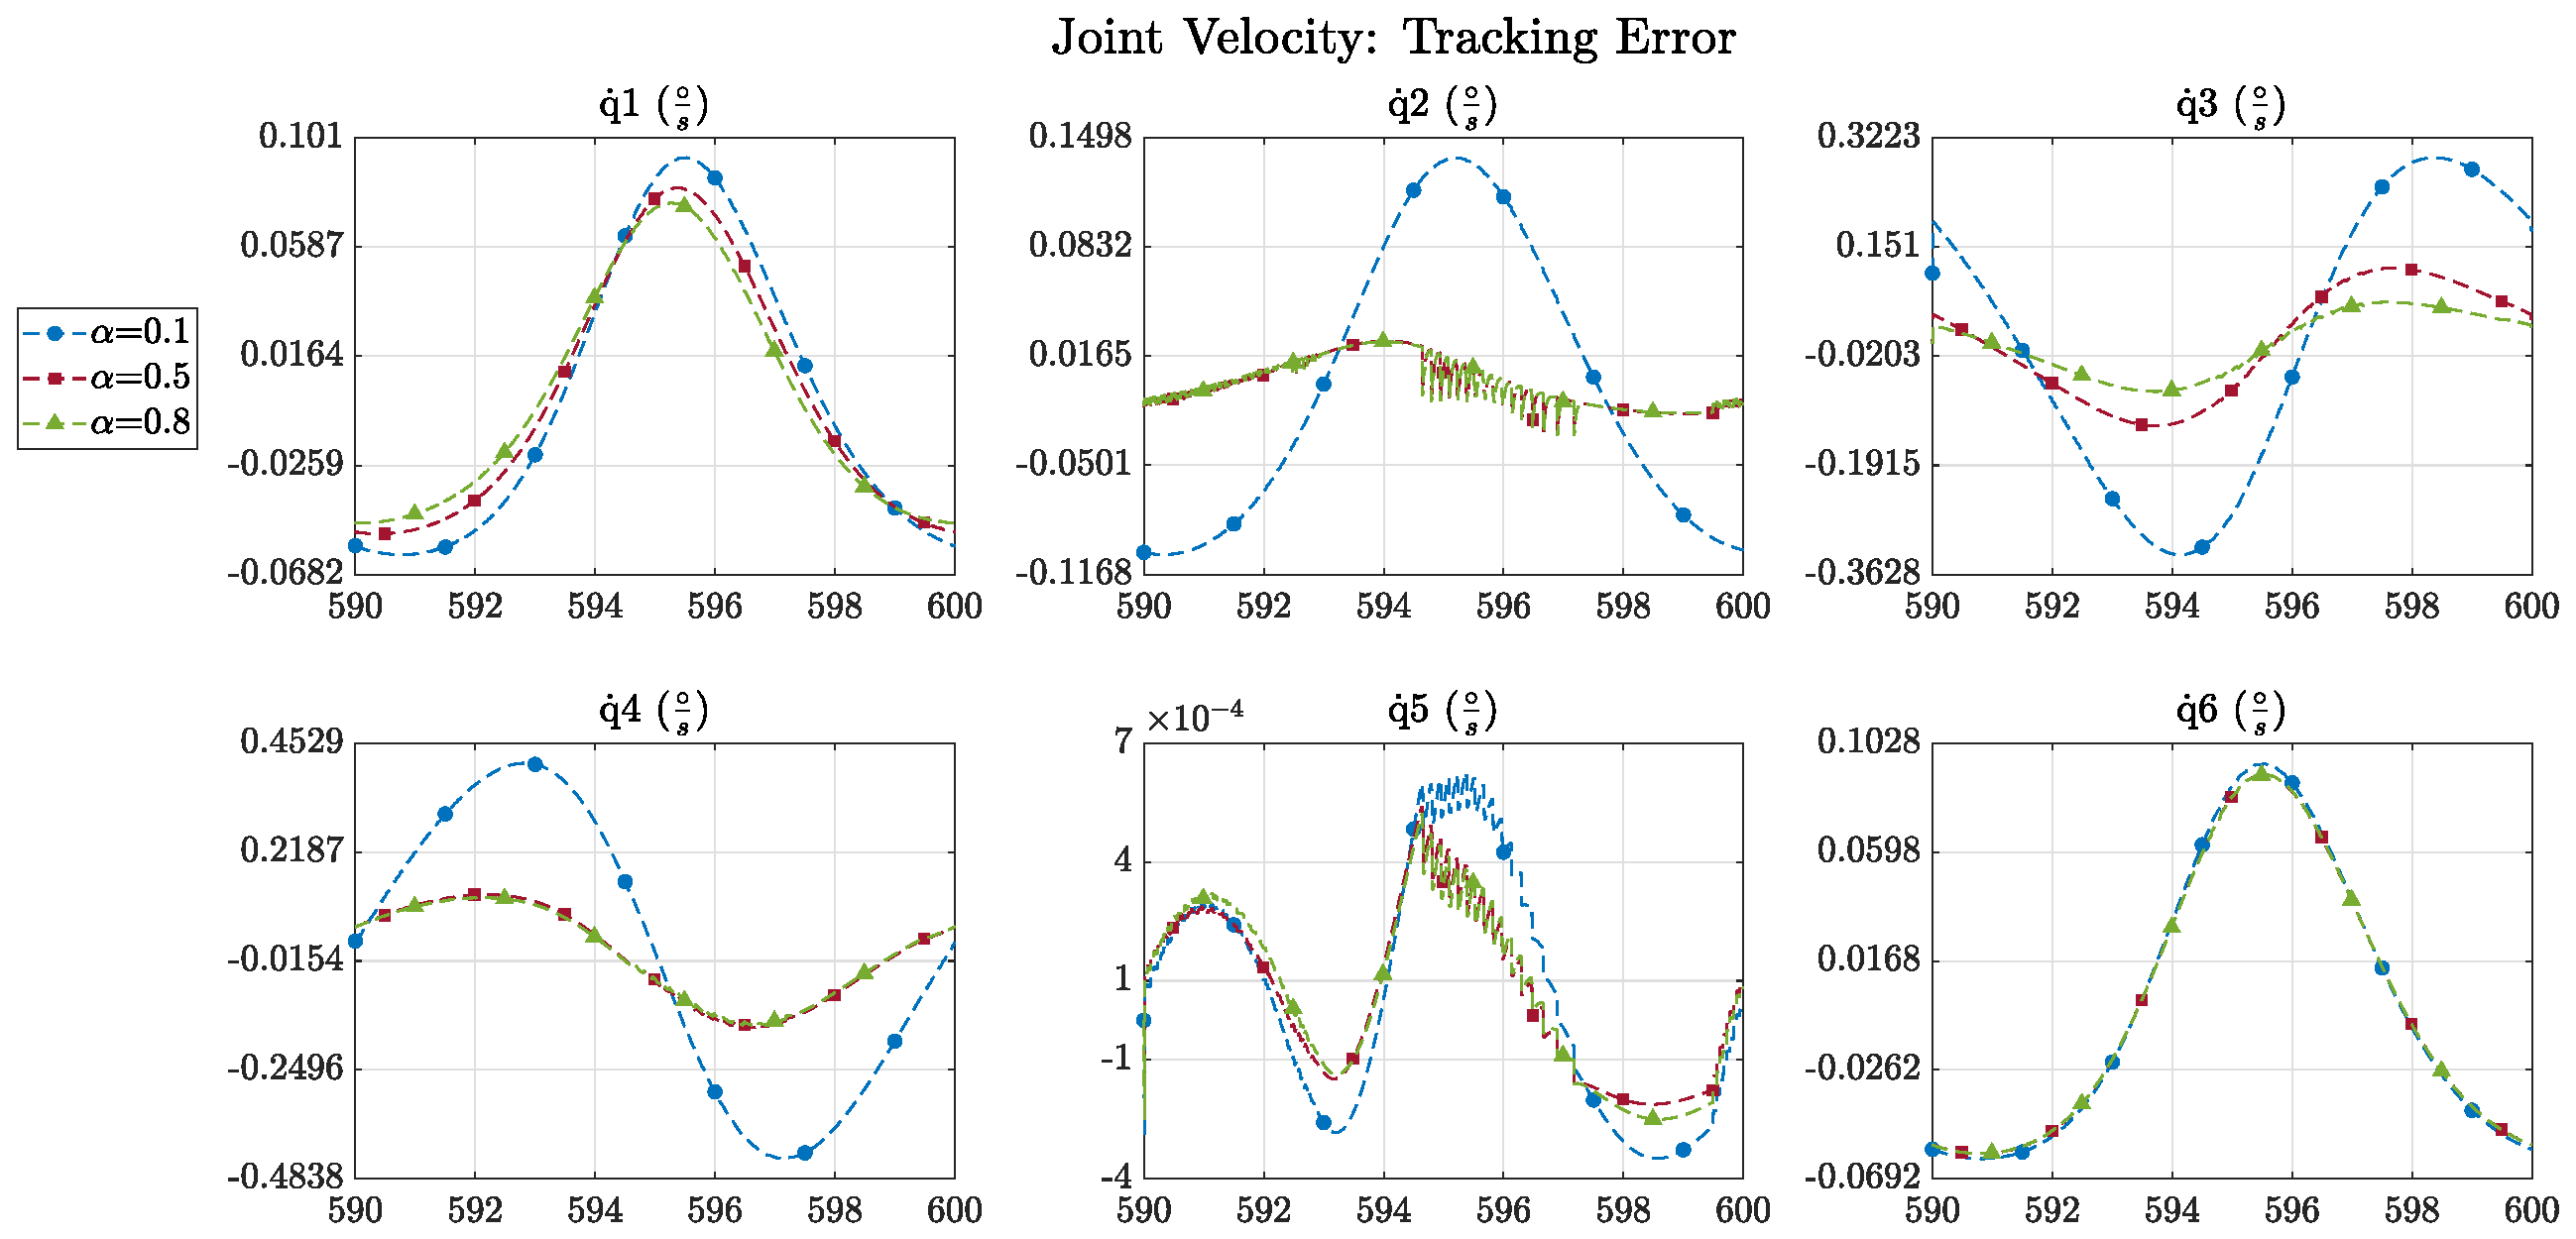
\includegraphics[width=1.1\textwidth]{img/SMCi/circular_traj/600_seg/articular_SMCi_velocity_error_compare.eps}
		\end{figure}
	\end{frame}
	
	\begin{frame}[fragile]{Control de modo deslizante}
		\begin{figure}
			\centering
			\hspace*{-0.5cm}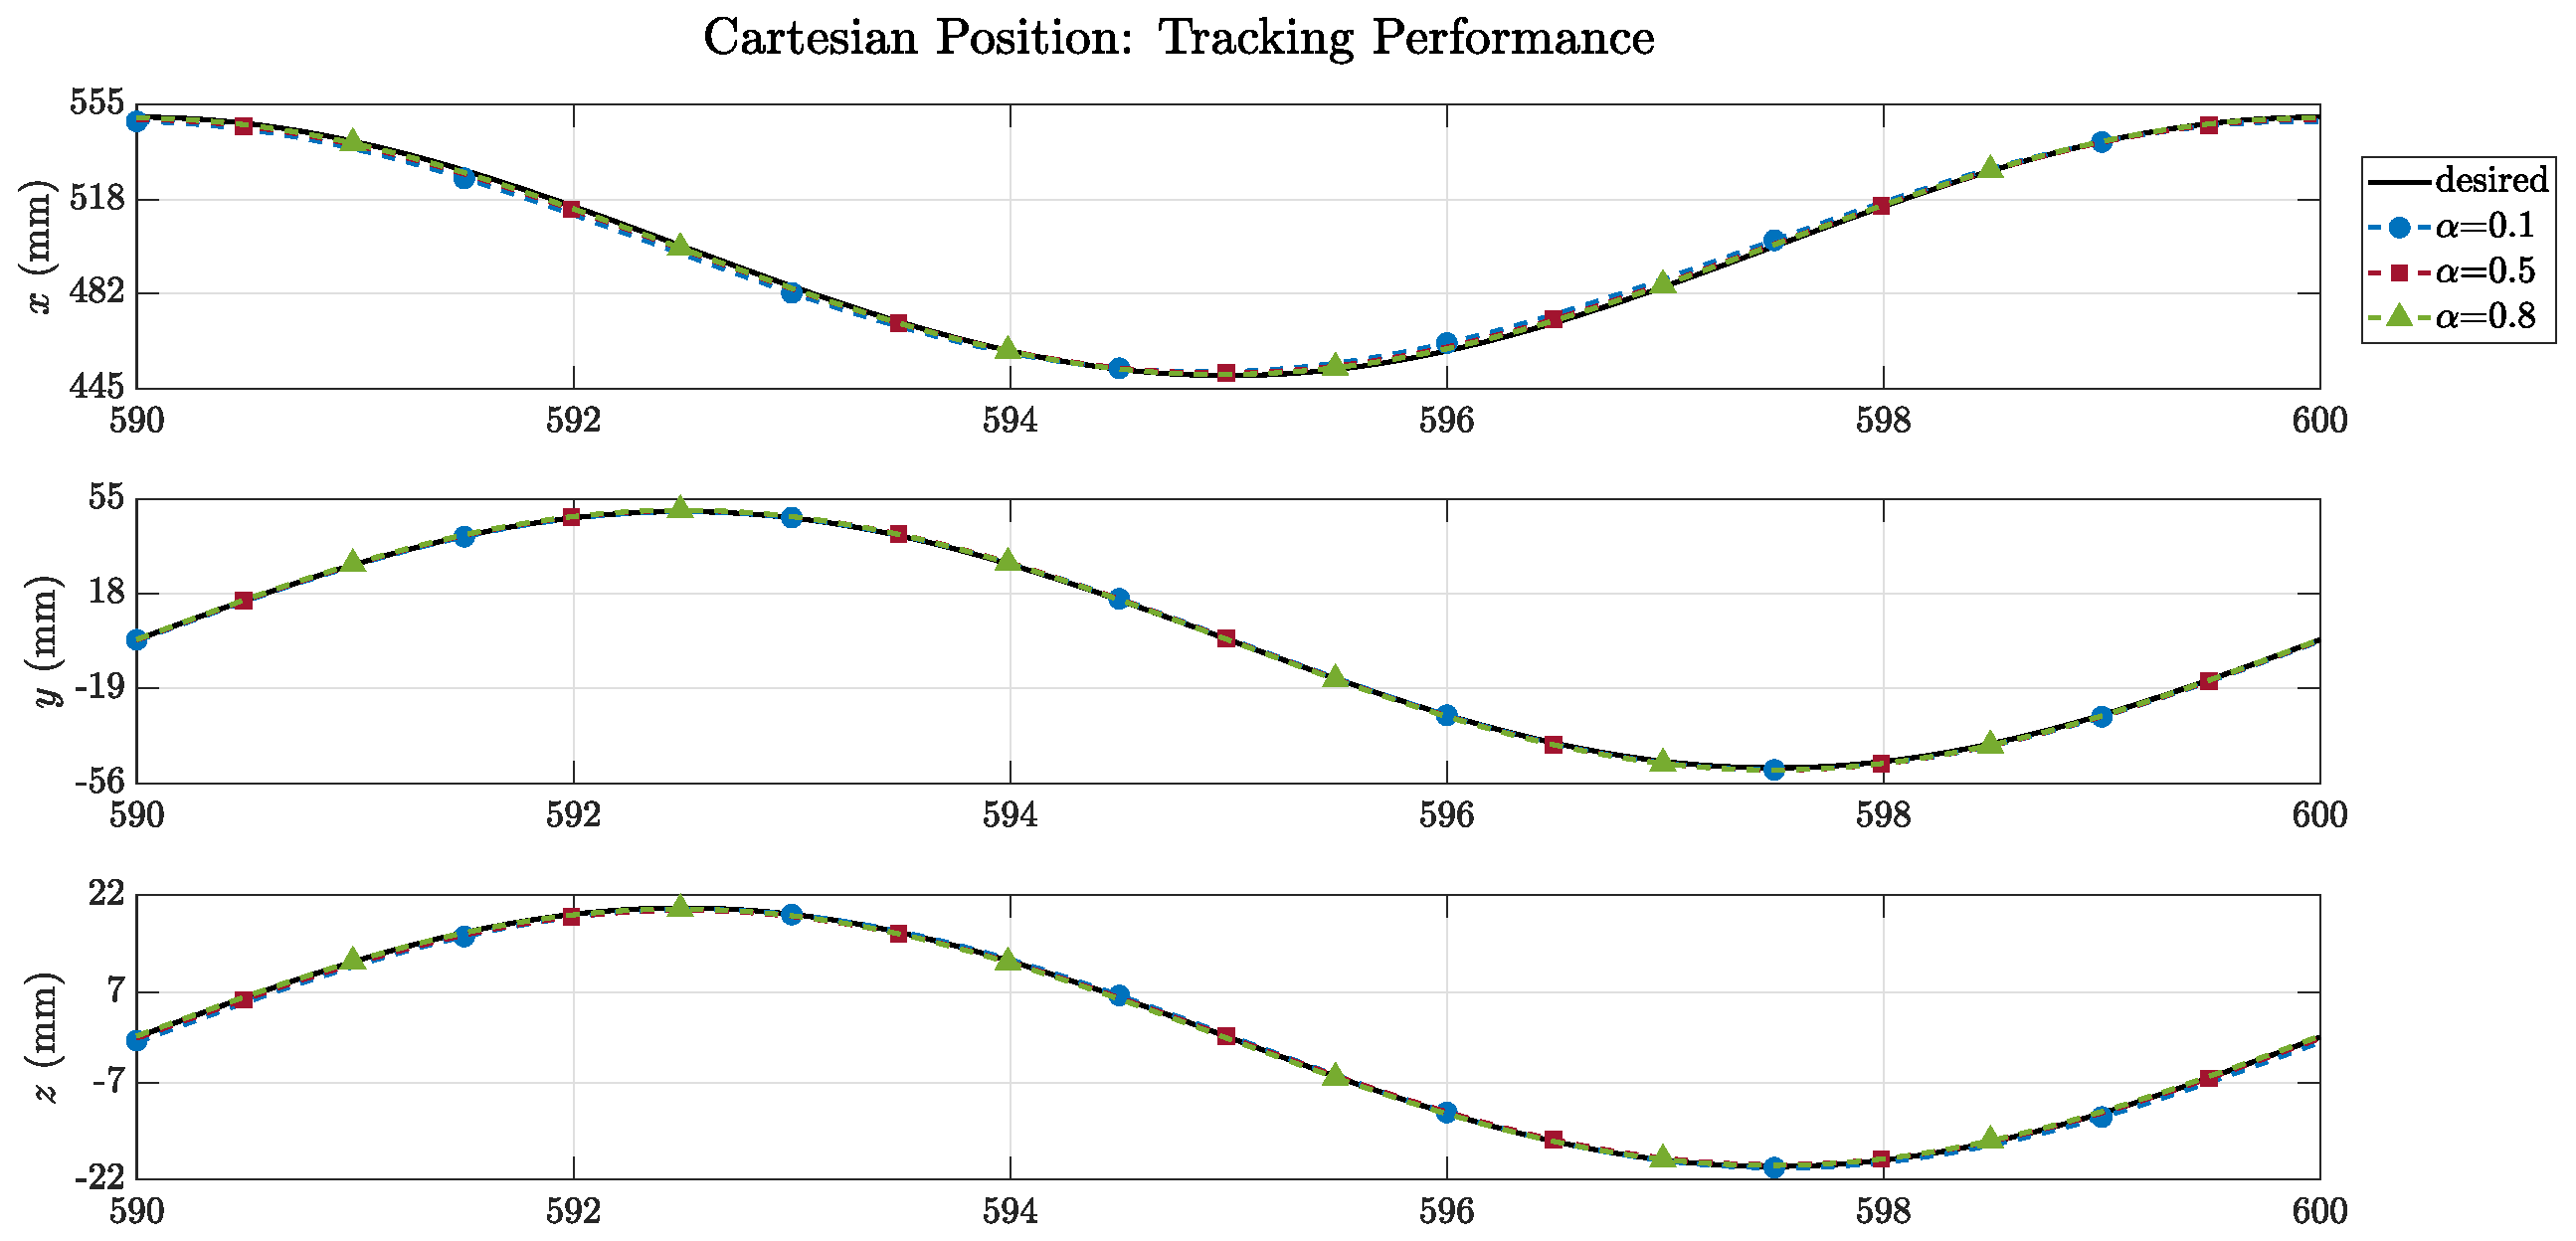
\includegraphics[width=1.1\textwidth]{img/SMCi/circular_traj/600_seg/articular_SMCi_pos_xyz_compare.eps}
		\end{figure}
	\end{frame}
	
	\begin{frame}[fragile]{Control de modo deslizante}
		\begin{figure}
			\centering
			\hspace*{-0.5cm}\includegraphics[width=1.1\textwidth]{img/SMCi/circular_traj/600_seg/articular_SMCi_pos_xyz_error_compare.eps}
		\end{figure}
	\end{frame}
	
	\begin{frame}[fragile]{Control de modo deslizante}
		\begin{figure}
			\centering
			\hspace*{-0.5cm}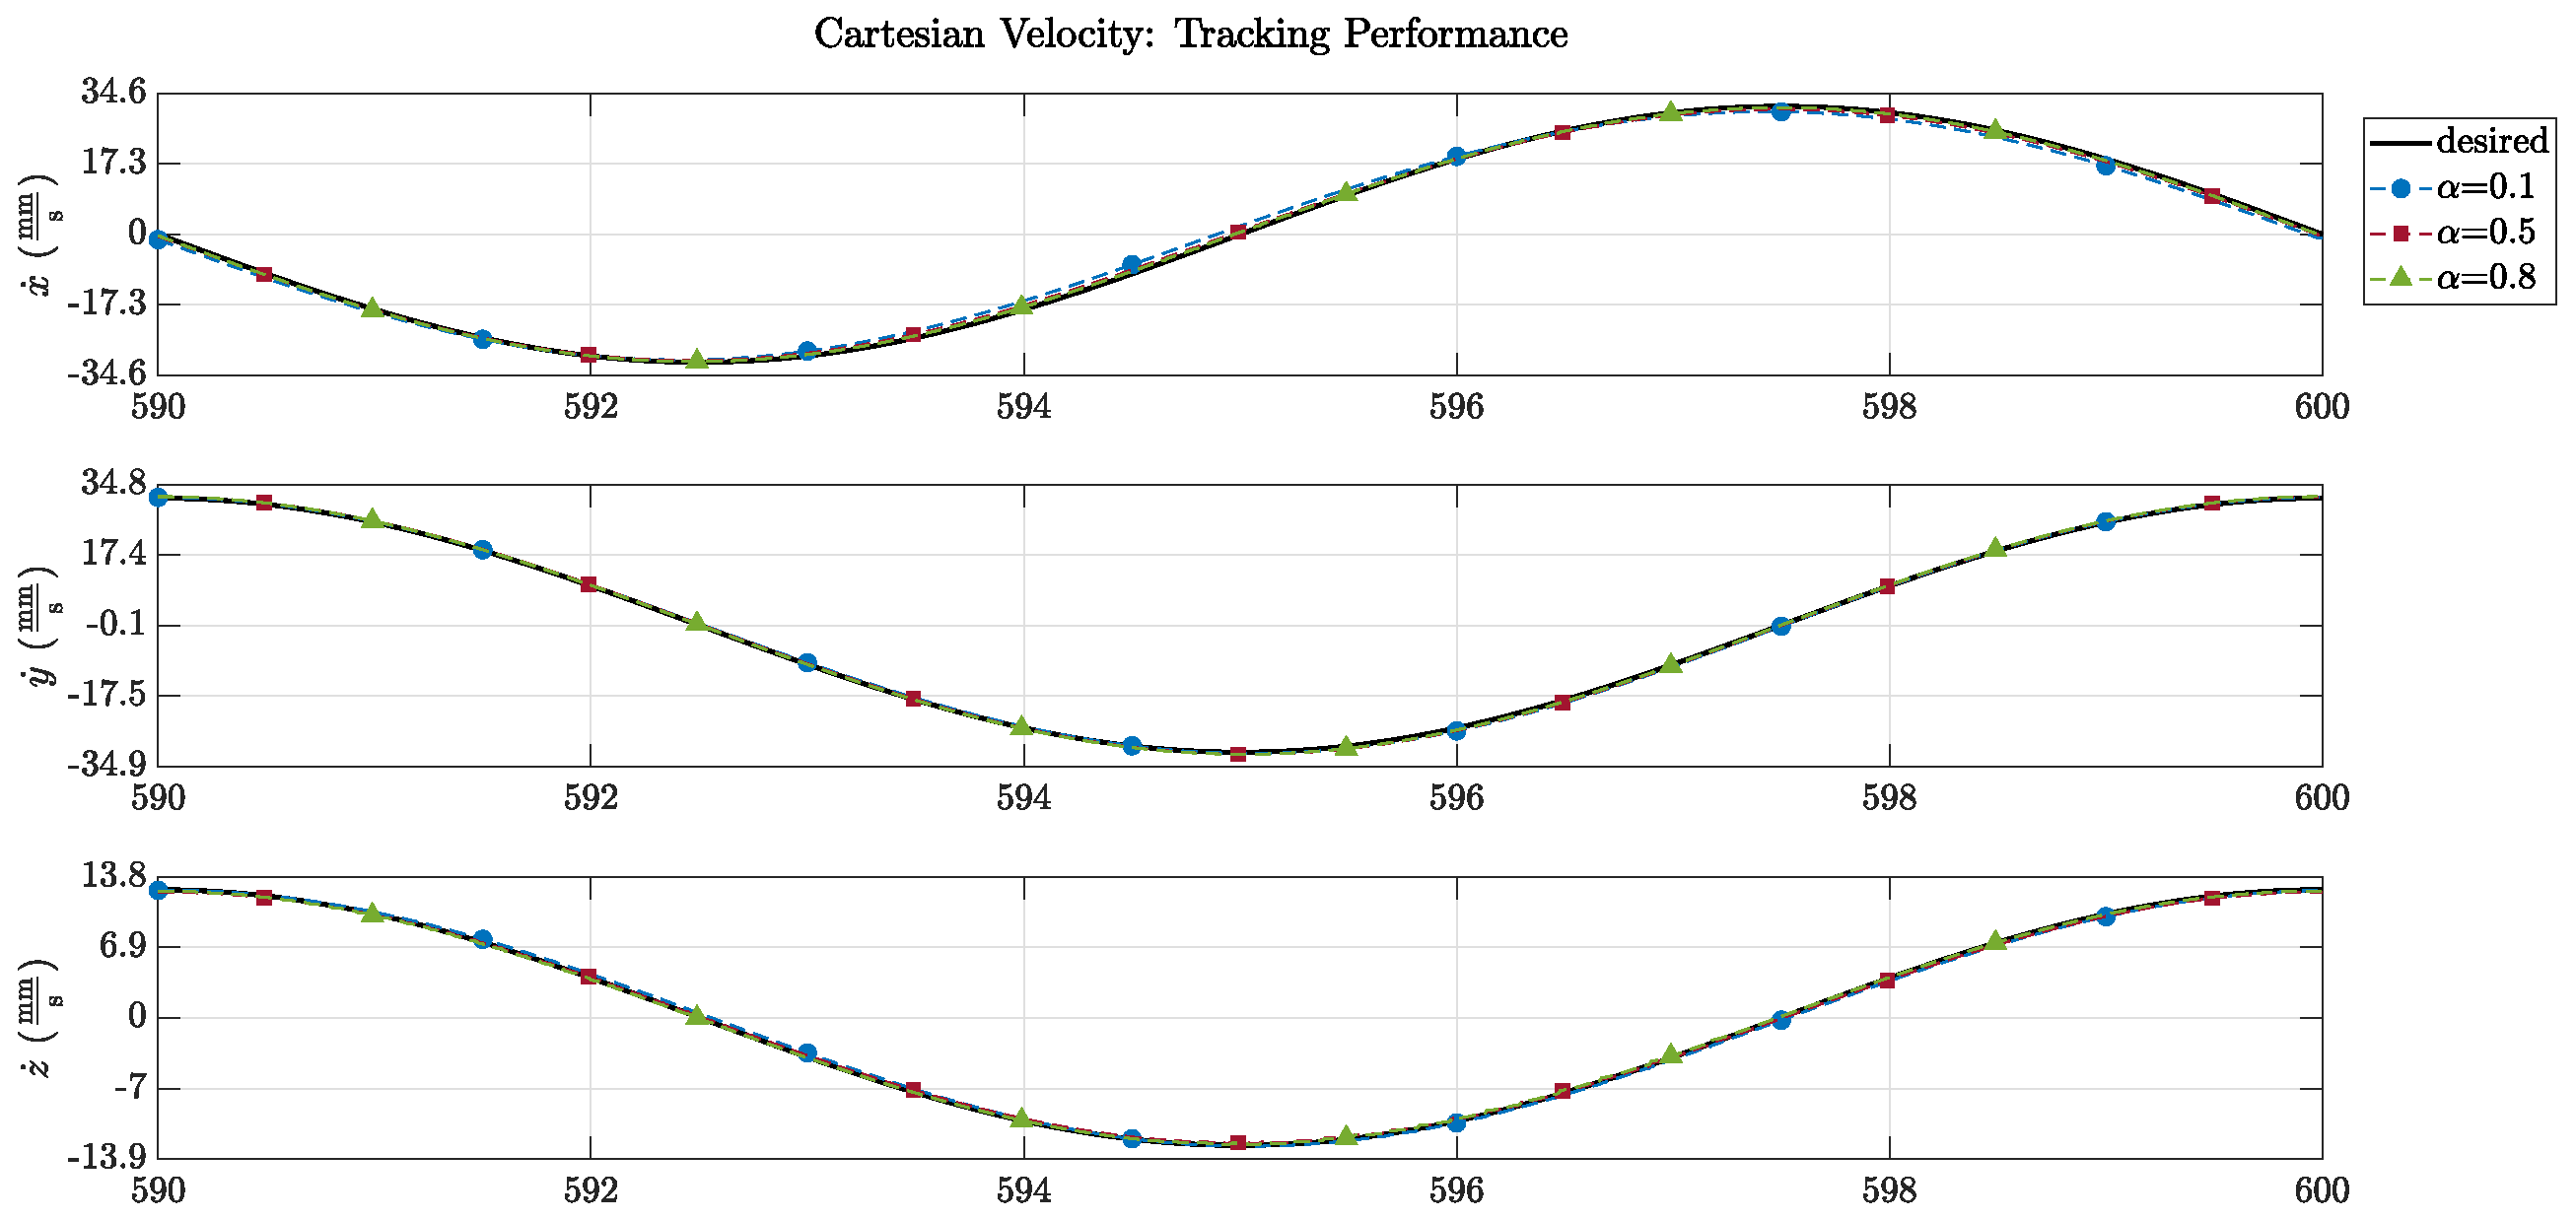
\includegraphics[width=1.1\textwidth]{img/SMCi/circular_traj/600_seg/articular_SMCi_vel_xyz_compare.eps}
		\end{figure}
	\end{frame}
	
	\begin{frame}[fragile]{Control de modo deslizante}
		\begin{figure}
			\centering
			\hspace*{-0.5cm}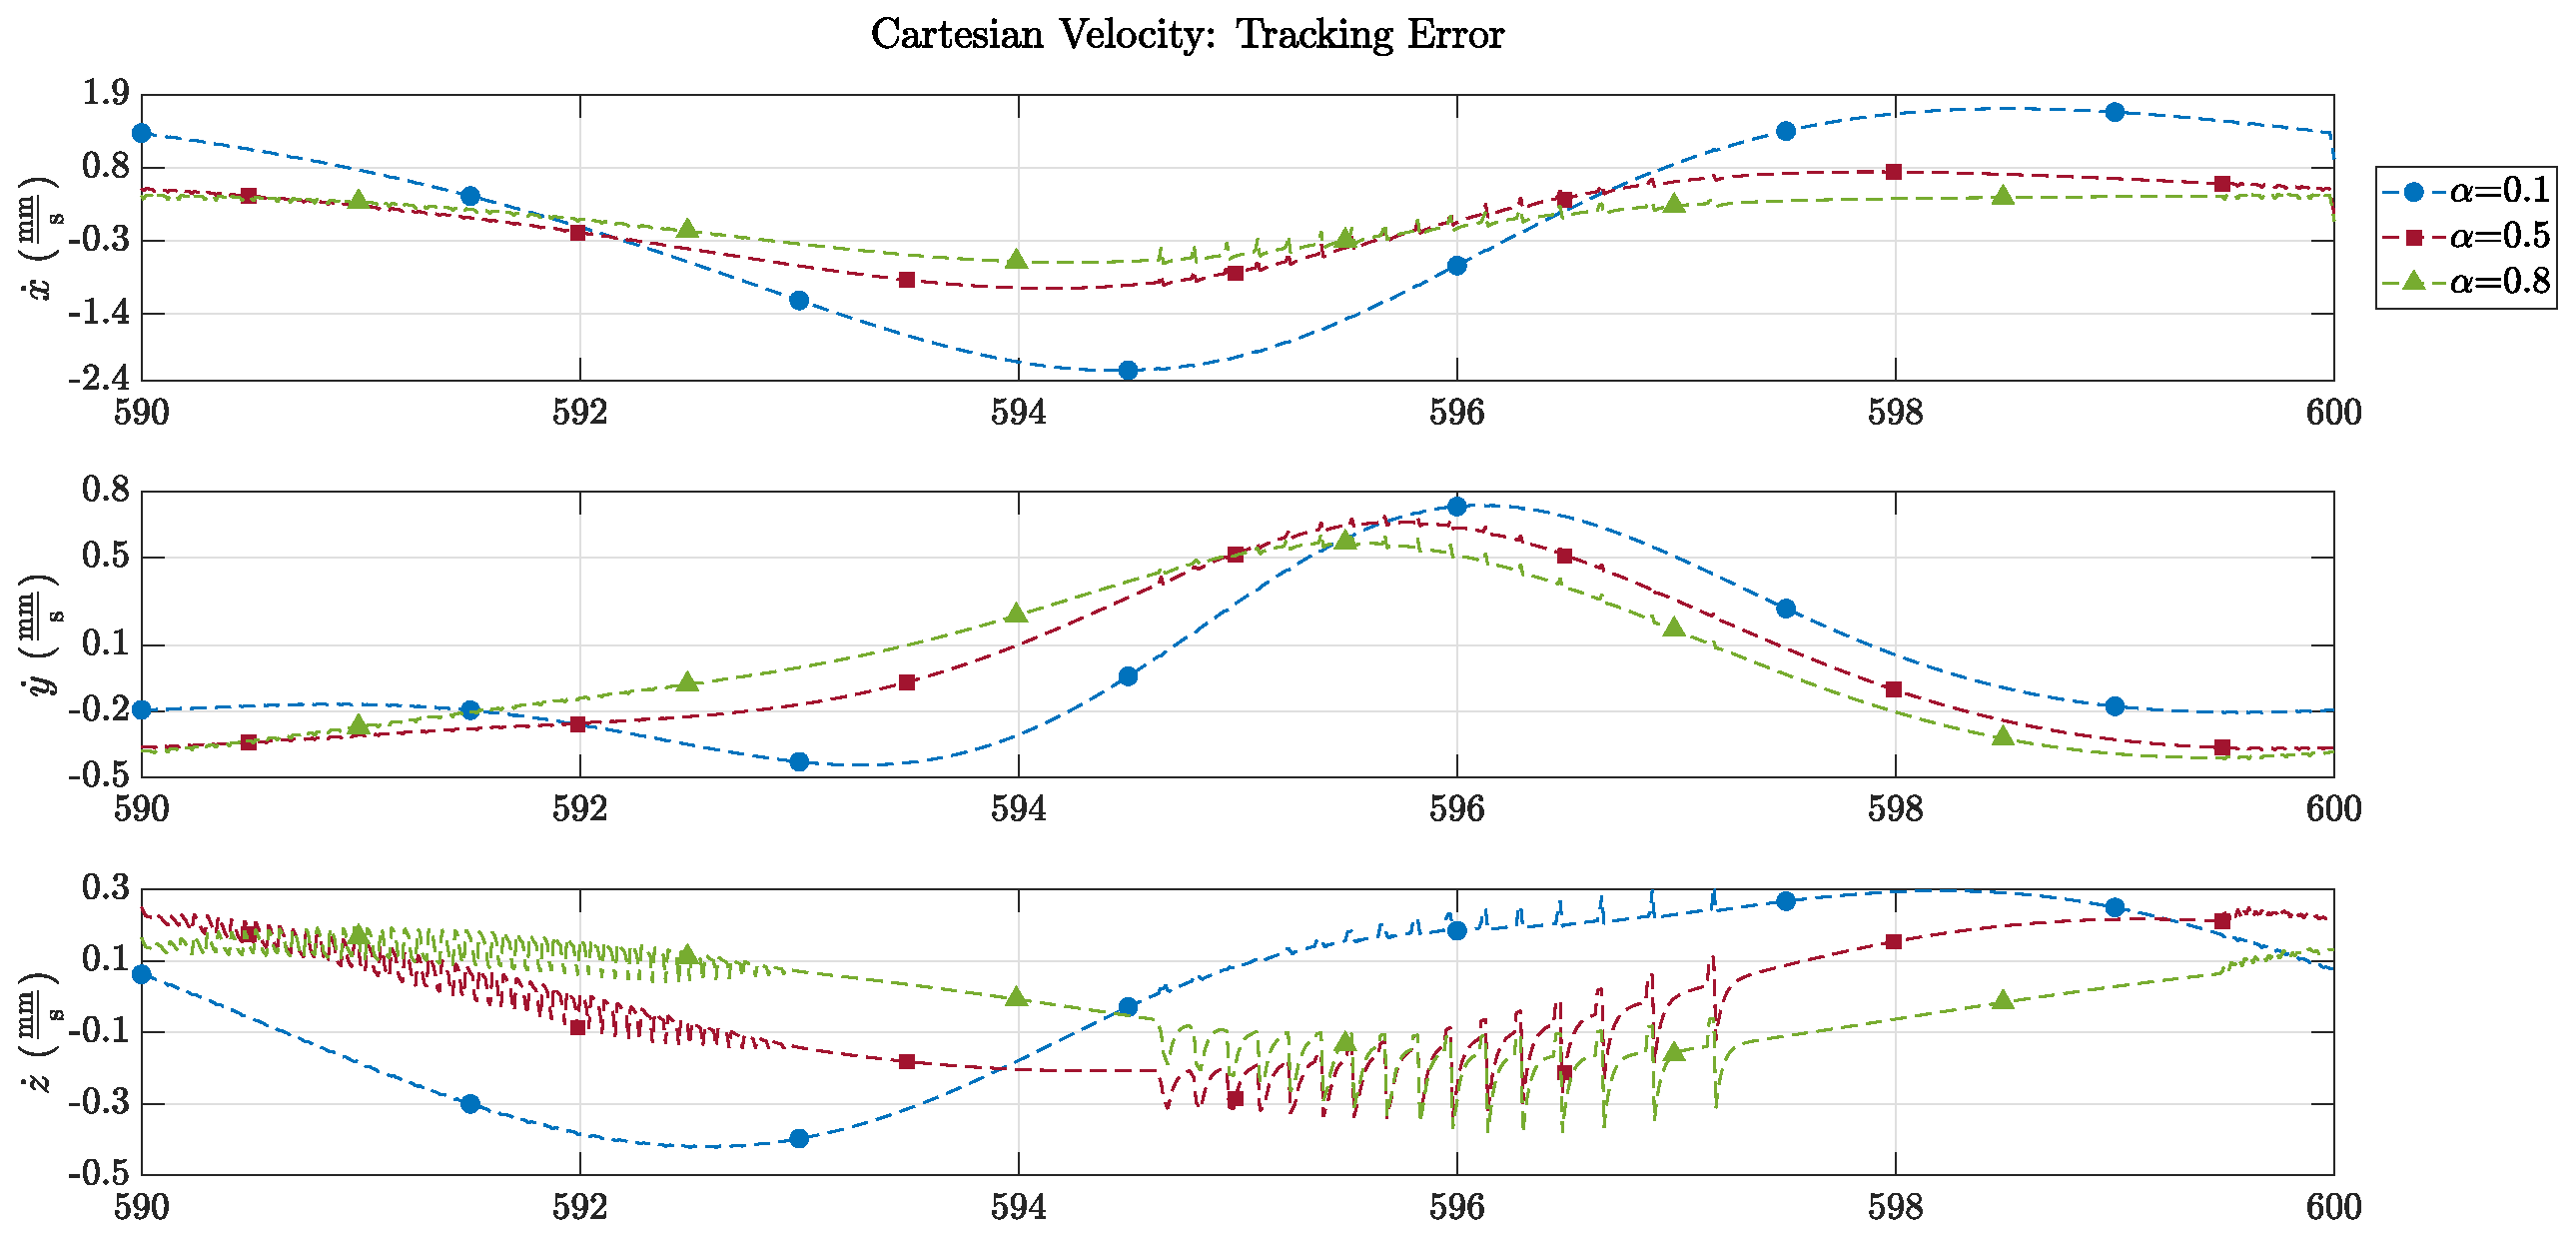
\includegraphics[width=1.1\textwidth]{img/SMCi/circular_traj/600_seg/articular_SMCi_vel_xyz_error_compare.eps}
		\end{figure}
	\end{frame}
	
	
	\begin{frame}[fragile]{Control de modo deslizante}
		\begin{figure}
			\centering
			\hspace*{-0.5cm}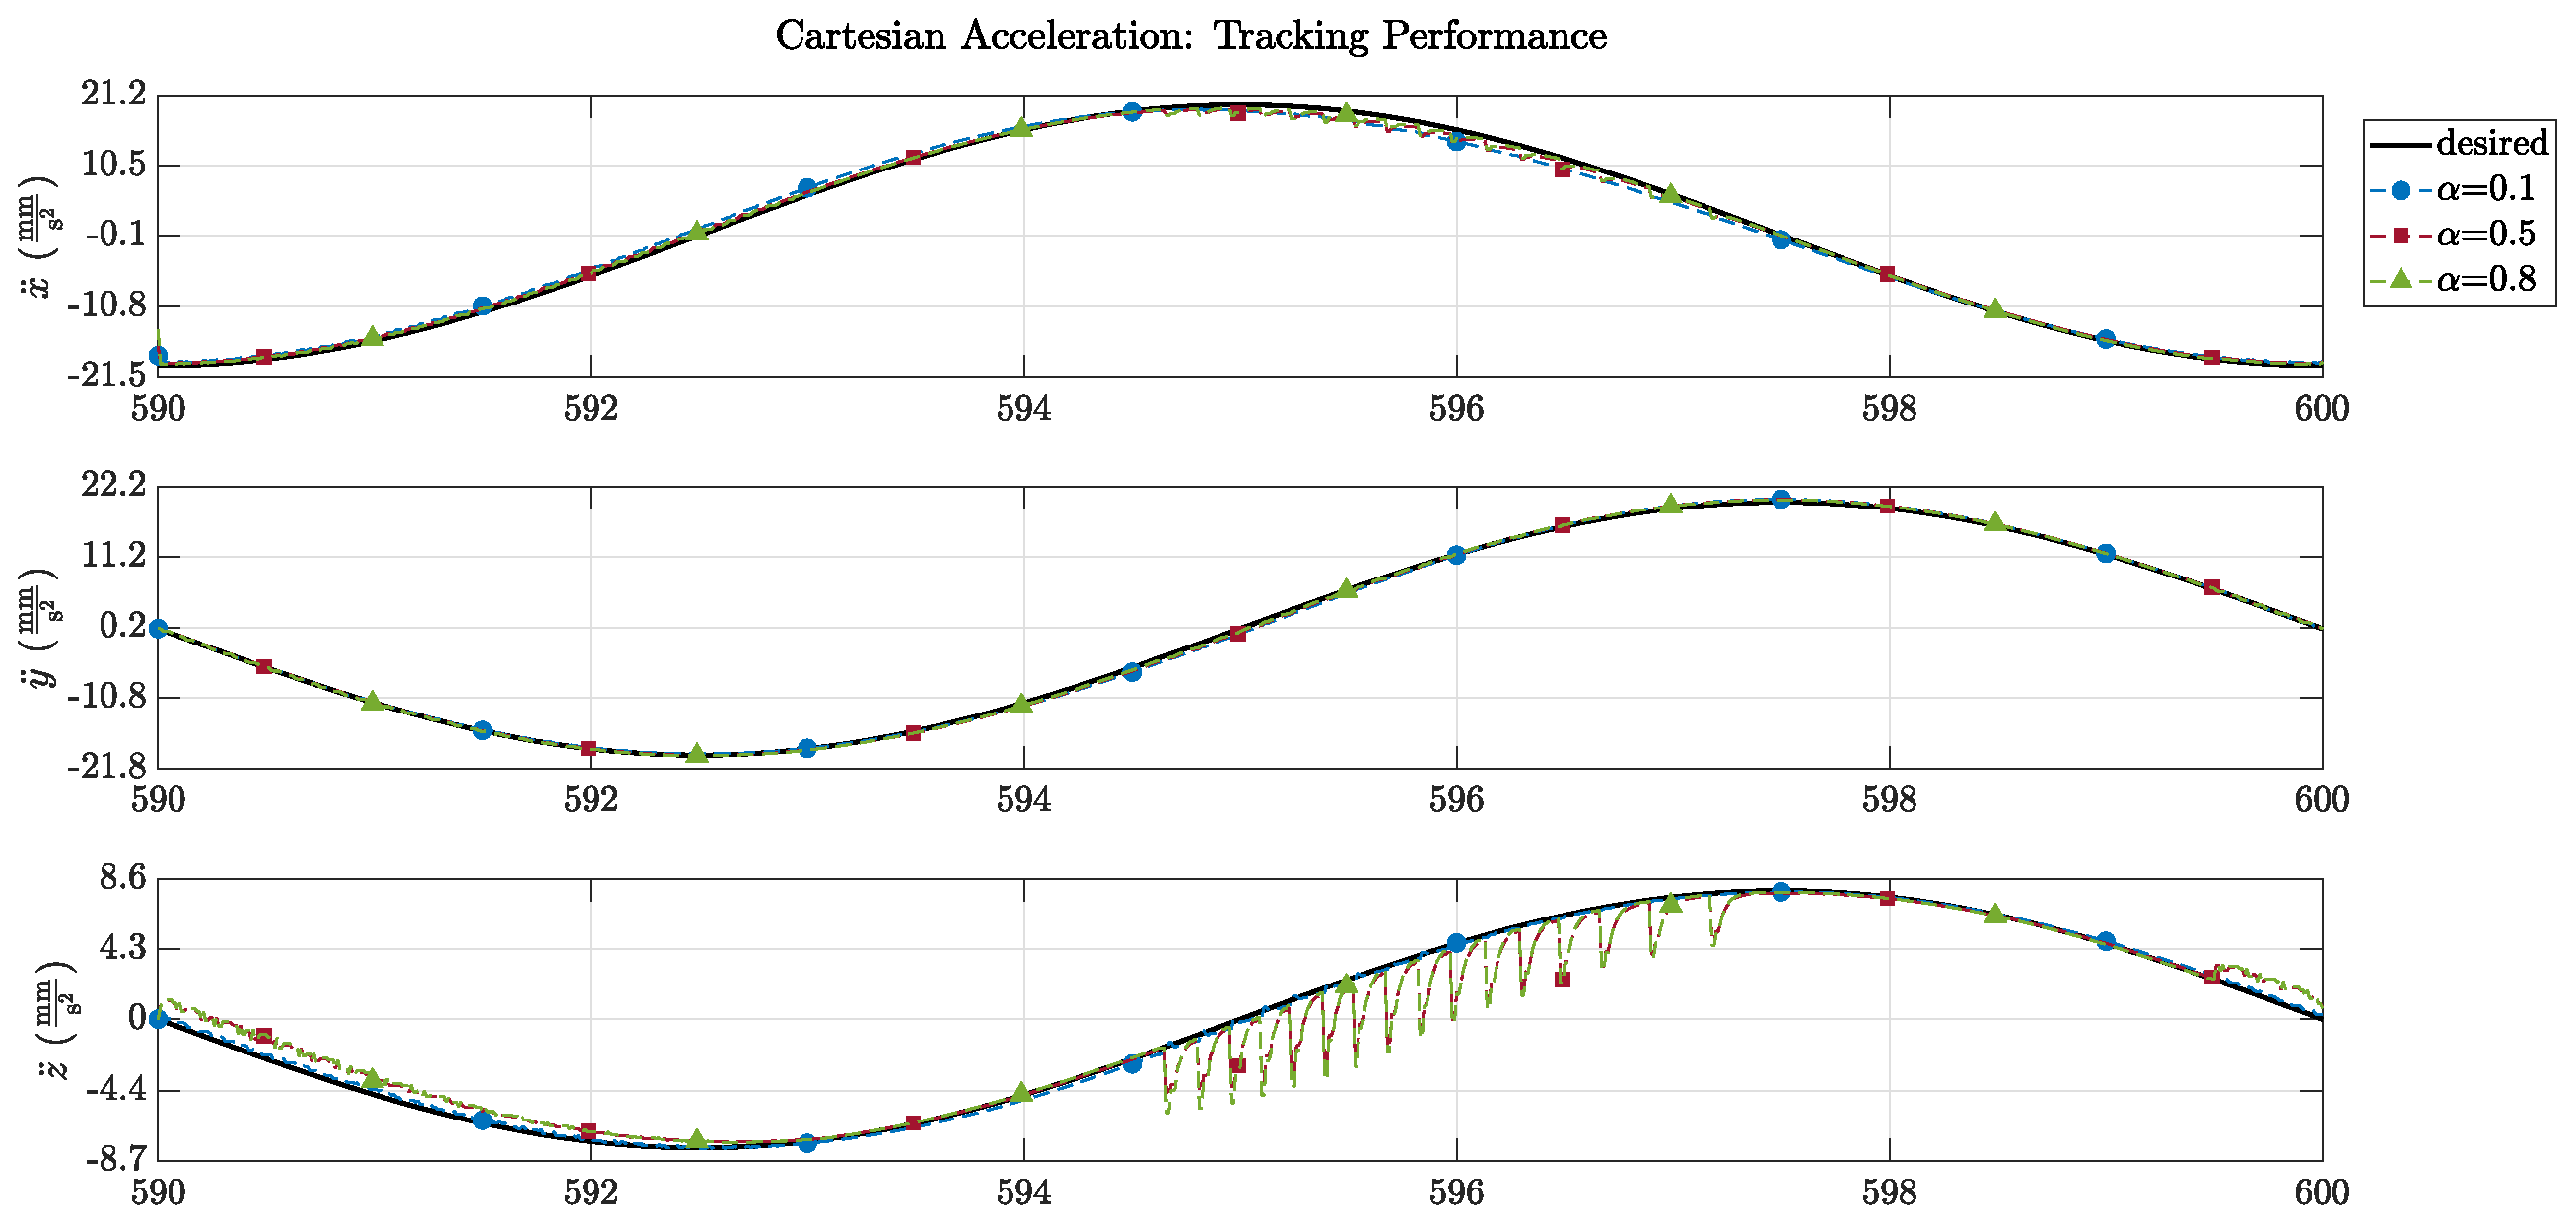
\includegraphics[width=1.1\textwidth]{img/SMCi/circular_traj/600_seg/articular_SMCi_accel_xyz_compare.eps}
		\end{figure}
	\end{frame}
	
	\begin{frame}[fragile]{Control de modo deslizante}
		\begin{figure}
			\centering
			\hspace*{-0.5cm}\includegraphics[width=1.1\textwidth]{img/SMCi/circular_traj/600_seg/articular_SMCi_accel_xyz_error_compare.eps}
		\end{figure}
	\end{frame}
	
	\begin{frame}[fragile]{Control de modo deslizante}
		\begin{figure}
			\centering
			\hspace*{-0.5cm}\includegraphics[width=1.1\textwidth]{img/SMCi/circular_traj/600_seg/articular_SMCi_jerk_xyz_compare.eps}
		\end{figure}
	\end{frame}
	
	\begin{frame}[fragile]{Control de modo deslizante}
		\begin{figure}
			\centering
			\hspace*{-0.5cm}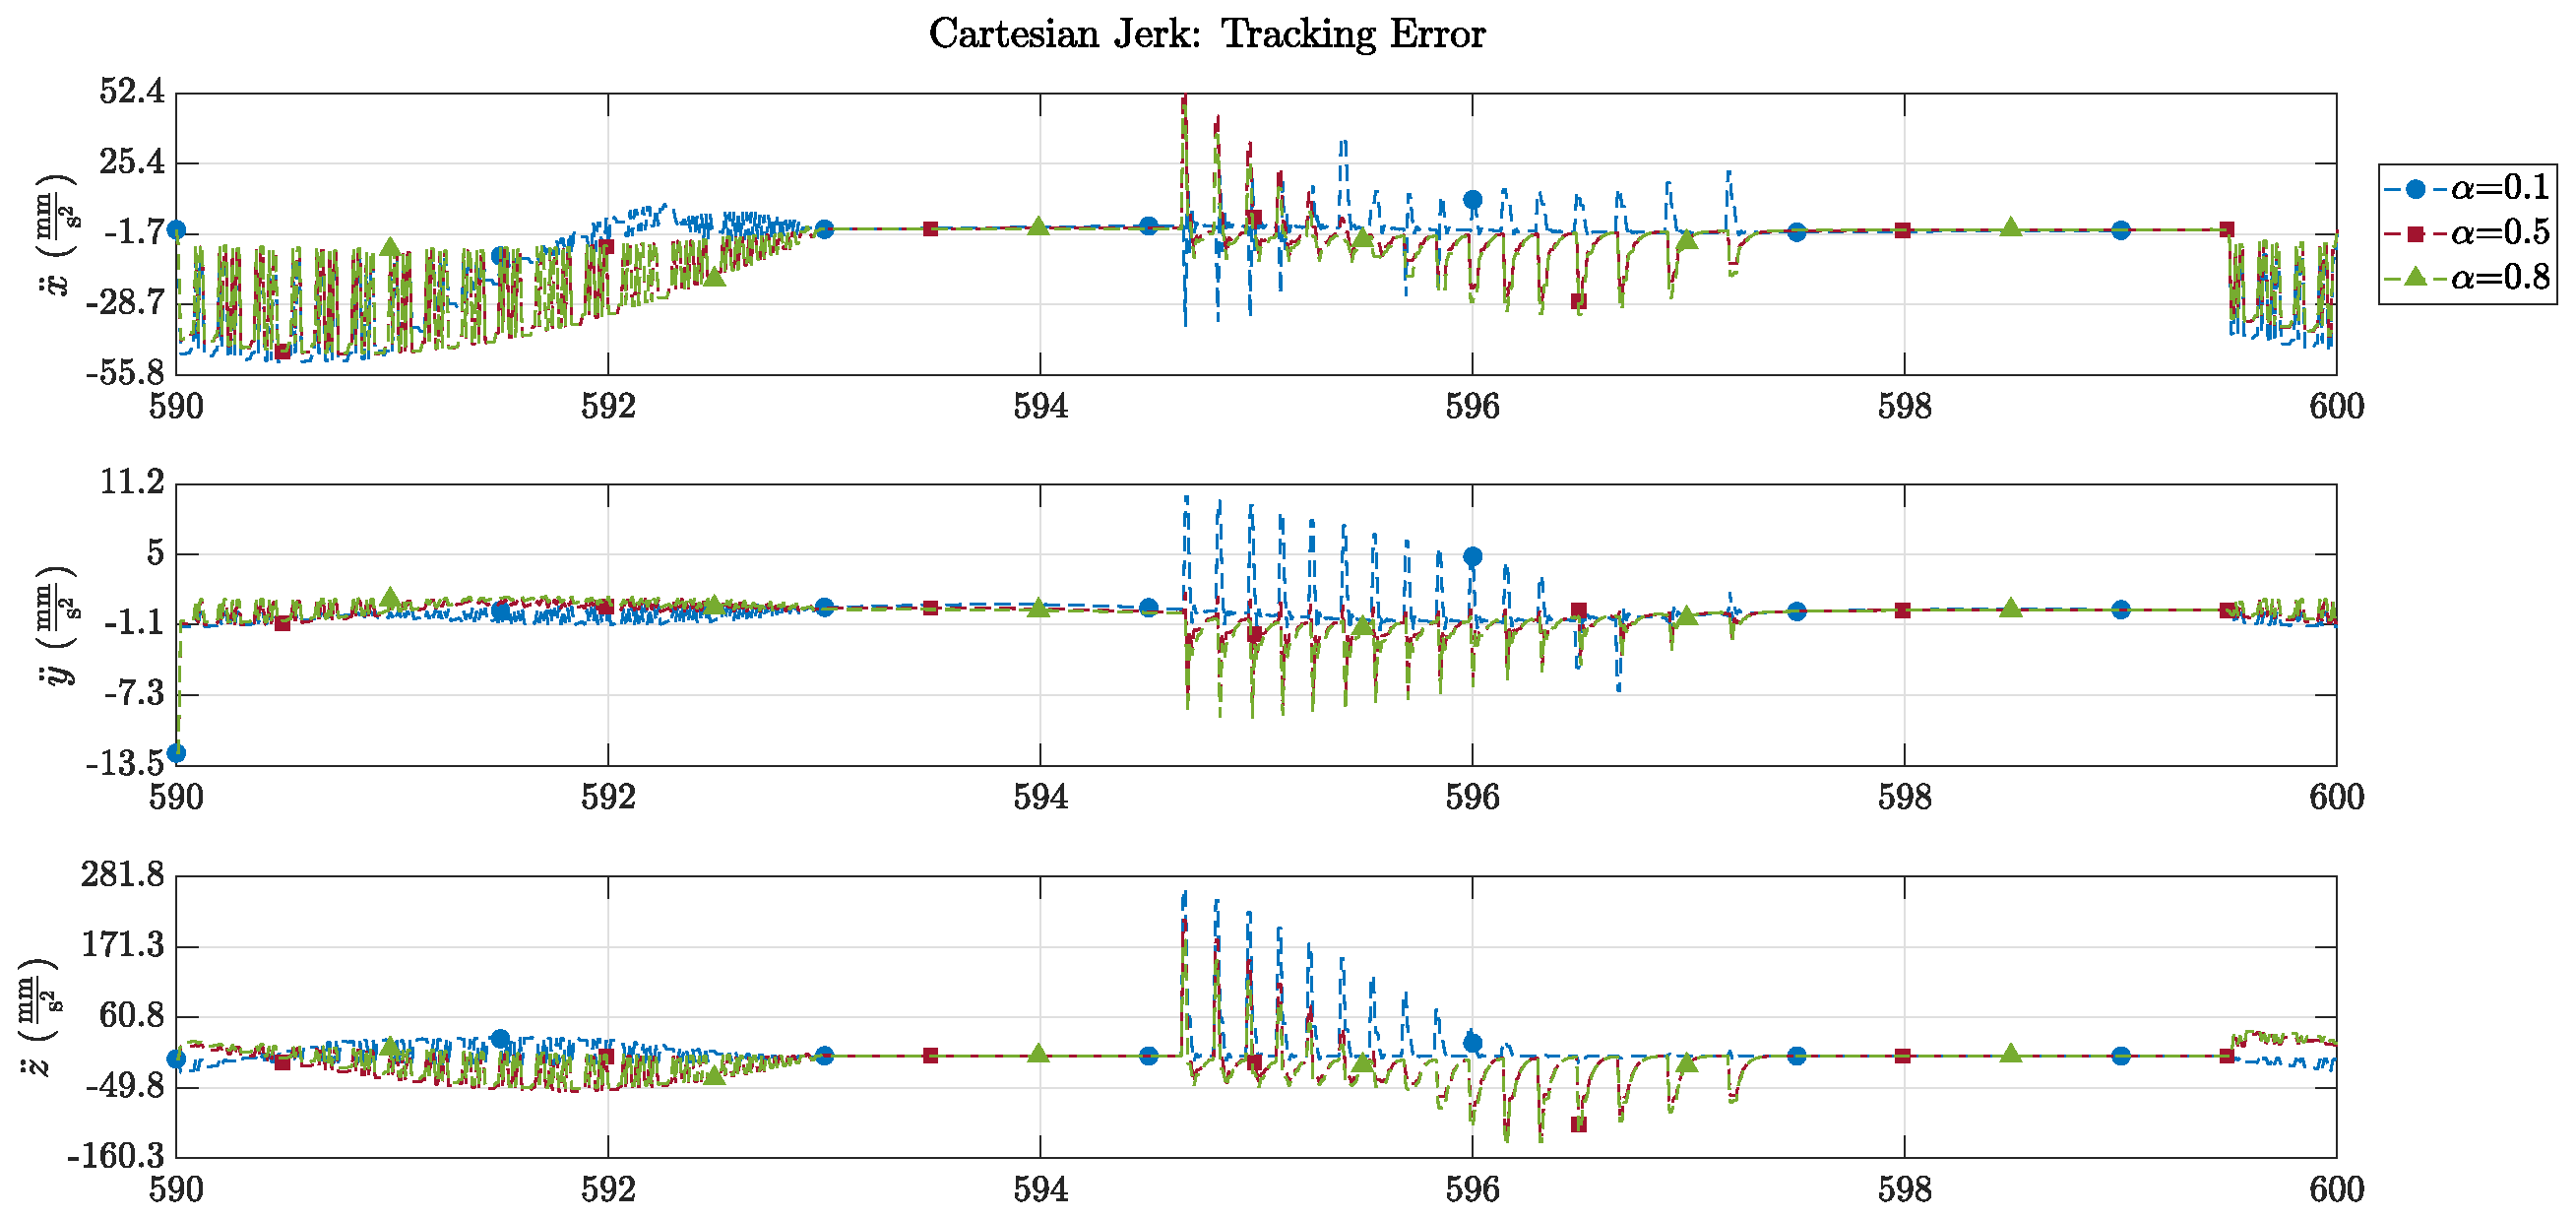
\includegraphics[width=1.1\textwidth]{img/SMCi/circular_traj/600_seg/articular_SMCi_jerk_xyz_error_compare.eps}
		\end{figure}
	\end{frame}
	
	\begin{frame}[fragile]{Control de modo deslizante}
		\begin{figure}
			\centering
			\hspace*{-0.5cm}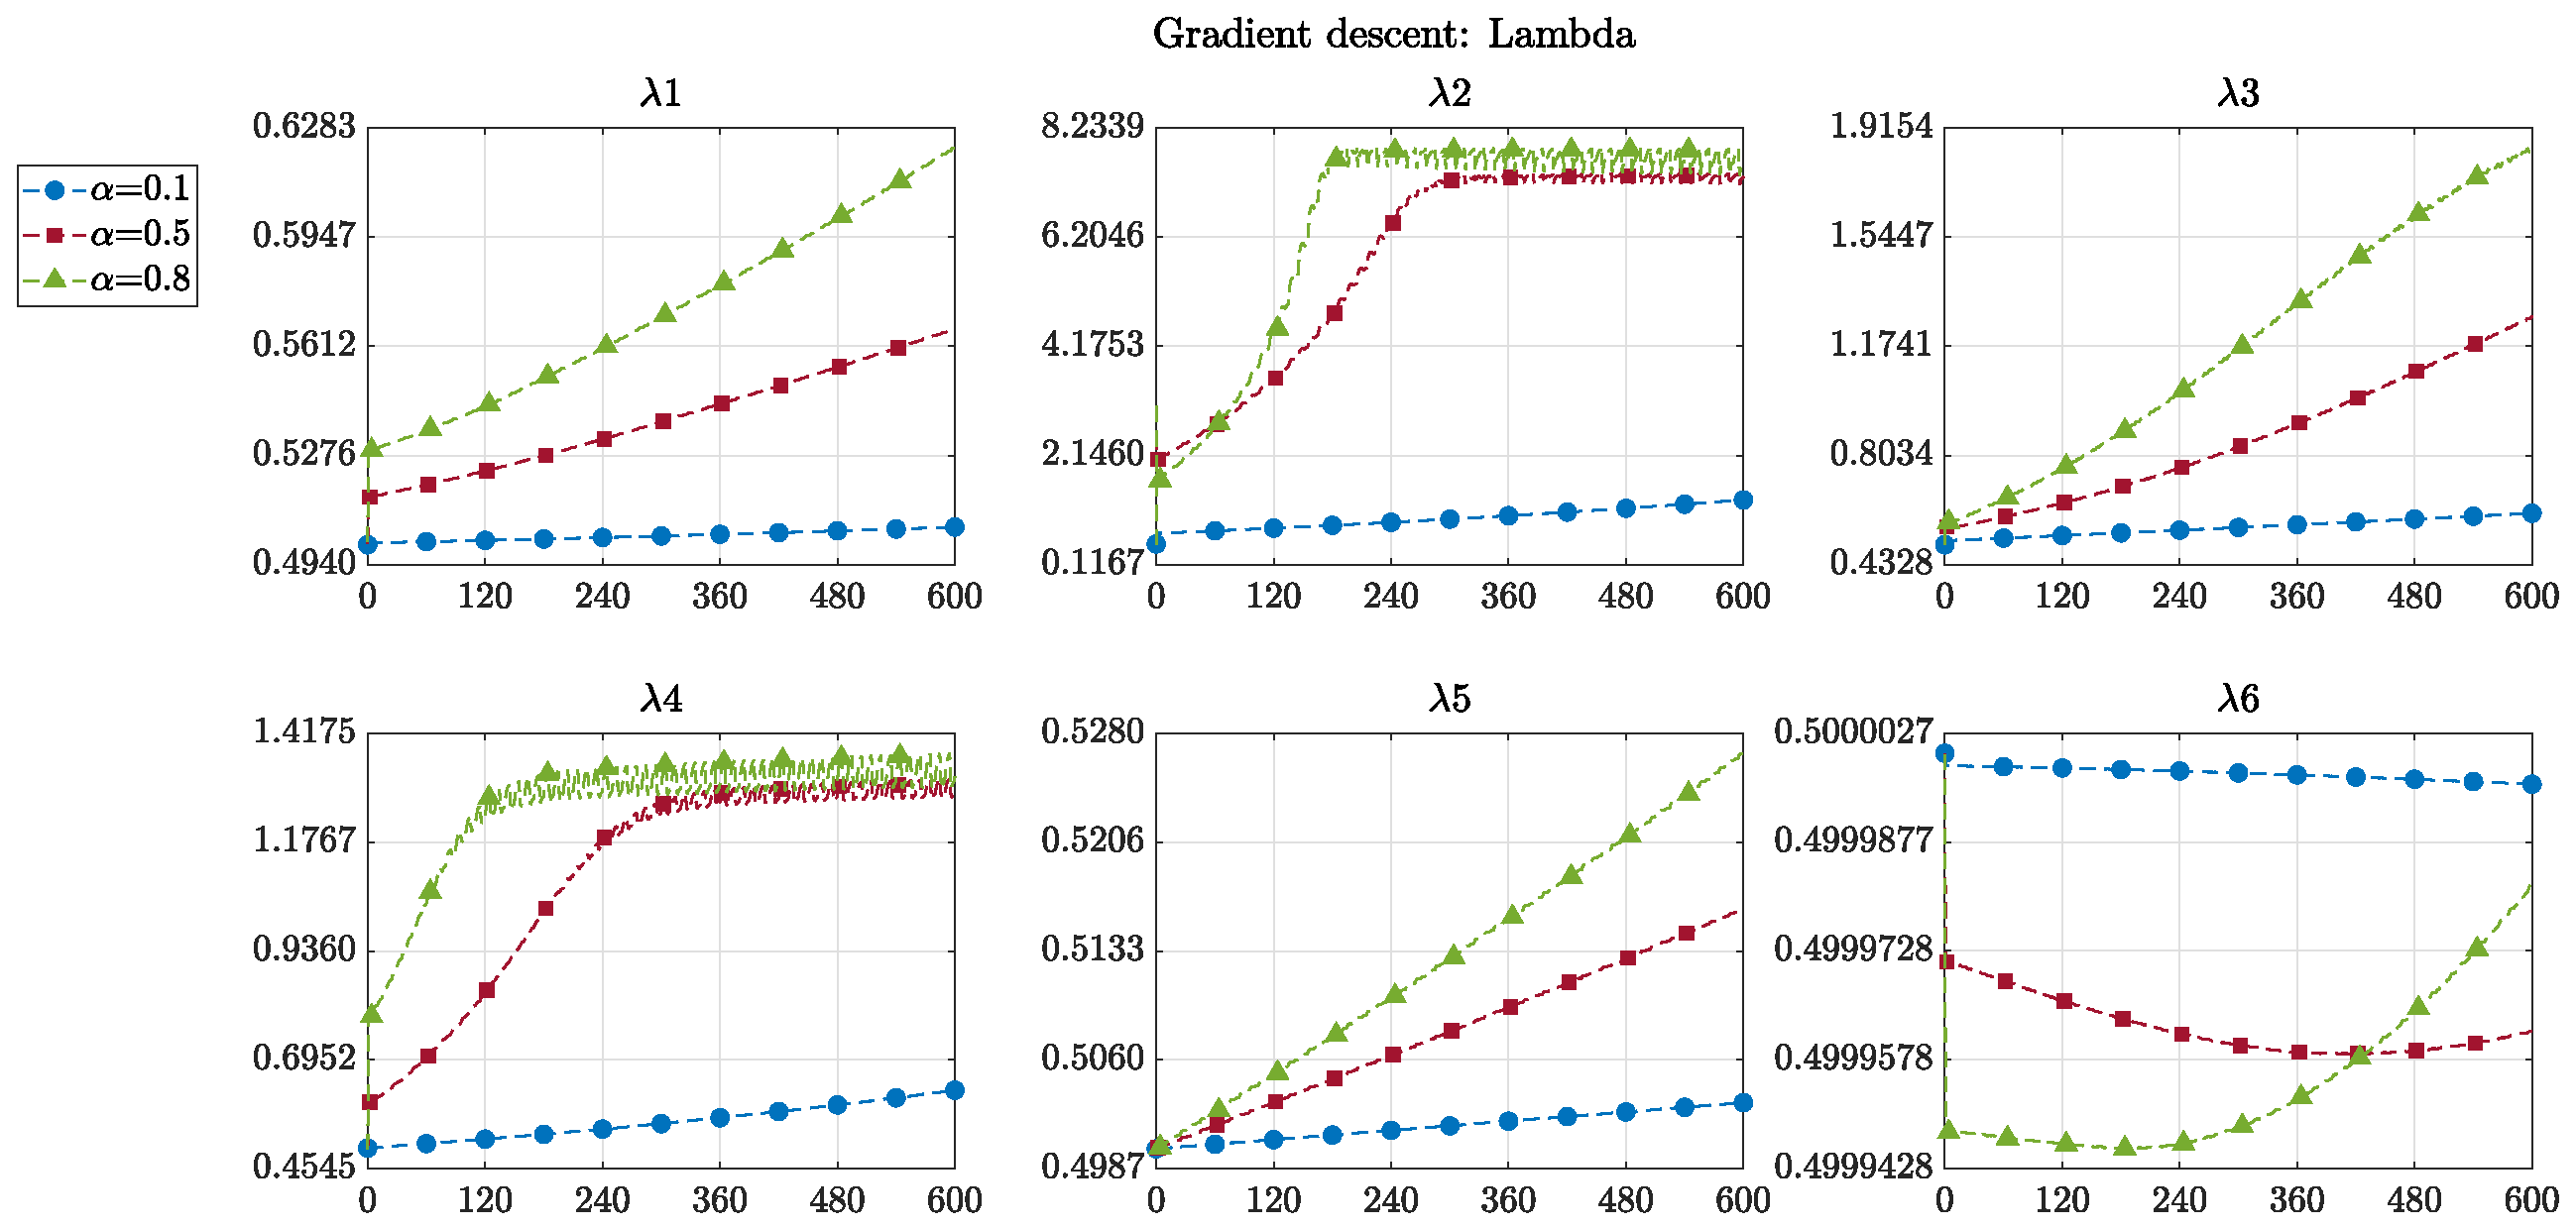
\includegraphics[width=1.1\textwidth]{img/SMCi/circular_traj/600_seg/articular_SMCi_lambda_compare.eps}
		\end{figure}
	\end{frame}
		
		
		
\end{document}
